\documentclass[twoside]{book}

% Packages required by doxygen
\usepackage{fixltx2e}
\usepackage{calc}
\usepackage{doxygen}
\usepackage[export]{adjustbox} % also loads graphicx
\usepackage{graphicx}
\usepackage[utf8]{inputenc}
\usepackage{makeidx}
\usepackage{multicol}
\usepackage{multirow}
\PassOptionsToPackage{warn}{textcomp}
\usepackage{textcomp}
\usepackage[nointegrals]{wasysym}
\usepackage[table]{xcolor}

% Font selection
\usepackage[T1]{fontenc}
\usepackage[scaled=.90]{helvet}
\usepackage{courier}
\usepackage{amssymb}
\usepackage{sectsty}
\renewcommand{\familydefault}{\sfdefault}
\allsectionsfont{%
  \fontseries{bc}\selectfont%
  \color{darkgray}%
}
\renewcommand{\DoxyLabelFont}{%
  \fontseries{bc}\selectfont%
  \color{darkgray}%
}
\newcommand{\+}{\discretionary{\mbox{\scriptsize$\hookleftarrow$}}{}{}}

% Page & text layout
\usepackage{geometry}
\geometry{%
  a4paper,%
  top=2.5cm,%
  bottom=2.5cm,%
  left=2.5cm,%
  right=2.5cm%
}
\tolerance=750
\hfuzz=15pt
\hbadness=750
\setlength{\emergencystretch}{15pt}
\setlength{\parindent}{0cm}
\setlength{\parskip}{3ex plus 2ex minus 2ex}
\makeatletter
\renewcommand{\paragraph}{%
  \@startsection{paragraph}{4}{0ex}{-1.0ex}{1.0ex}{%
    \normalfont\normalsize\bfseries\SS@parafont%
  }%
}
\renewcommand{\subparagraph}{%
  \@startsection{subparagraph}{5}{0ex}{-1.0ex}{1.0ex}{%
    \normalfont\normalsize\bfseries\SS@subparafont%
  }%
}
\makeatother

% Headers & footers
\usepackage{fancyhdr}
\pagestyle{fancyplain}
\fancyhead[LE]{\fancyplain{}{\bfseries\thepage}}
\fancyhead[CE]{\fancyplain{}{}}
\fancyhead[RE]{\fancyplain{}{\bfseries\leftmark}}
\fancyhead[LO]{\fancyplain{}{\bfseries\rightmark}}
\fancyhead[CO]{\fancyplain{}{}}
\fancyhead[RO]{\fancyplain{}{\bfseries\thepage}}
\fancyfoot[LE]{\fancyplain{}{}}
\fancyfoot[CE]{\fancyplain{}{}}
\fancyfoot[RE]{\fancyplain{}{\bfseries\scriptsize Generated by Doxygen }}
\fancyfoot[LO]{\fancyplain{}{\bfseries\scriptsize Generated by Doxygen }}
\fancyfoot[CO]{\fancyplain{}{}}
\fancyfoot[RO]{\fancyplain{}{}}
\renewcommand{\footrulewidth}{0.4pt}
\renewcommand{\chaptermark}[1]{%
  \markboth{#1}{}%
}
\renewcommand{\sectionmark}[1]{%
  \markright{\thesection\ #1}%
}

% Indices & bibliography
\usepackage{natbib}
\usepackage[titles]{tocloft}
\setcounter{tocdepth}{3}
\setcounter{secnumdepth}{5}
\makeindex

% Custom commands
\newcommand{\clearemptydoublepage}{%
  \newpage{\pagestyle{empty}\cleardoublepage}%
}

\usepackage{caption}
\captionsetup{labelsep=space,justification=centering,font={bf},singlelinecheck=off,skip=4pt,position=top}

%===== C O N T E N T S =====

\begin{document}

% Titlepage & ToC
\pagenumbering{alph}
\begin{titlepage}
\vspace*{7cm}
\begin{center}%
{\Large Life }\\
\vspace*{1cm}
{\large Generated by Doxygen 1.8.13}\\
\end{center}
\end{titlepage}
\clearemptydoublepage
\pagenumbering{roman}
\tableofcontents
\clearemptydoublepage
\pagenumbering{arabic}

%--- Begin generated contents ---
\chapter{Hierarchical Index}
\section{Class Hierarchy}
This inheritance list is sorted roughly, but not completely, alphabetically\+:\begin{DoxyCompactList}
\item \contentsline{section}{Cell}{\pageref{classCell}}{}
\item \contentsline{section}{Organism\+:\+:Coordinates}{\pageref{structOrganism_1_1Coordinates}}{}
\item \contentsline{section}{Grid}{\pageref{classGrid}}{}
\item \contentsline{section}{Organism}{\pageref{classOrganism}}{}
\begin{DoxyCompactList}
\item \contentsline{section}{Ant}{\pageref{classAnt}}{}
\item \contentsline{section}{Doodlebug}{\pageref{classDoodlebug}}{}
\end{DoxyCompactList}
\item \contentsline{section}{Production}{\pageref{classProduction}}{}
\item \contentsline{section}{Tests2}{\pageref{classTests2}}{}
\end{DoxyCompactList}

\chapter{Data Structure Index}
\section{Data Structures}
Here are the data structures with brief descriptions\+:\begin{DoxyCompactList}
\item\contentsline{section}{\textbf{ Ant} }{\pageref{classAnt}}{}
\item\contentsline{section}{\textbf{ Cell} }{\pageref{classCell}}{}
\item\contentsline{section}{\textbf{ Organism\+::\+Coordinates} }{\pageref{structOrganism_1_1Coordinates}}{}
\item\contentsline{section}{\textbf{ Doodlebug} }{\pageref{classDoodlebug}}{}
\item\contentsline{section}{\textbf{ Grid} }{\pageref{classGrid}}{}
\item\contentsline{section}{\textbf{ Organism} }{\pageref{classOrganism}}{}
\item\contentsline{section}{\textbf{ Production} }{\pageref{classProduction}}{}
\item\contentsline{section}{\textbf{ Tests2} }{\pageref{classTests2}}{}
\end{DoxyCompactList}

\chapter{File Index}
\section{File List}
Here is a list of all files with brief descriptions\+:\begin{DoxyCompactList}
\item\contentsline{section}{\textbf{ Ant.\+cpp} }{\pageref{Ant_8cpp}}{}
\item\contentsline{section}{\textbf{ Ant.\+h} }{\pageref{Ant_8h}}{}
\item\contentsline{section}{\textbf{ Ants\+And\+Doodles.\+cpp} }{\pageref{AntsAndDoodles_8cpp}}{}
\item\contentsline{section}{\textbf{ Cell.\+cpp} }{\pageref{Cell_8cpp}}{}
\item\contentsline{section}{\textbf{ Cell.\+h} }{\pageref{Cell_8h}}{}
\item\contentsline{section}{\textbf{ Doodlebug.\+cpp} }{\pageref{Doodlebug_8cpp}}{}
\item\contentsline{section}{\textbf{ Doodlebug.\+h} }{\pageref{Doodlebug_8h}}{}
\item\contentsline{section}{\textbf{ Grid.\+cpp} }{\pageref{Grid_8cpp}}{}
\item\contentsline{section}{\textbf{ Grid.\+h} }{\pageref{Grid_8h}}{}
\item\contentsline{section}{\textbf{ Organism.\+cpp} }{\pageref{Organism_8cpp}}{}
\item\contentsline{section}{\textbf{ Organism.\+h} }{\pageref{Organism_8h}}{}
\item\contentsline{section}{\textbf{ Production.\+cpp} }{\pageref{Production_8cpp}}{}
\item\contentsline{section}{\textbf{ Production.\+h} }{\pageref{Production_8h}}{}
\item\contentsline{section}{\textbf{ Tests2.\+cpp} }{\pageref{Tests2_8cpp}}{}
\item\contentsline{section}{\textbf{ Tests2.\+h} }{\pageref{Tests2_8h}}{}
\end{DoxyCompactList}

\chapter{Data Structure Documentation}
\section{Ant Class Reference}
\label{classAnt}\index{Ant@{Ant}}


{\ttfamily \#include $<$Ant.\+h$>$}

Inheritance diagram for Ant\+:\begin{figure}[H]
\begin{center}
\leavevmode
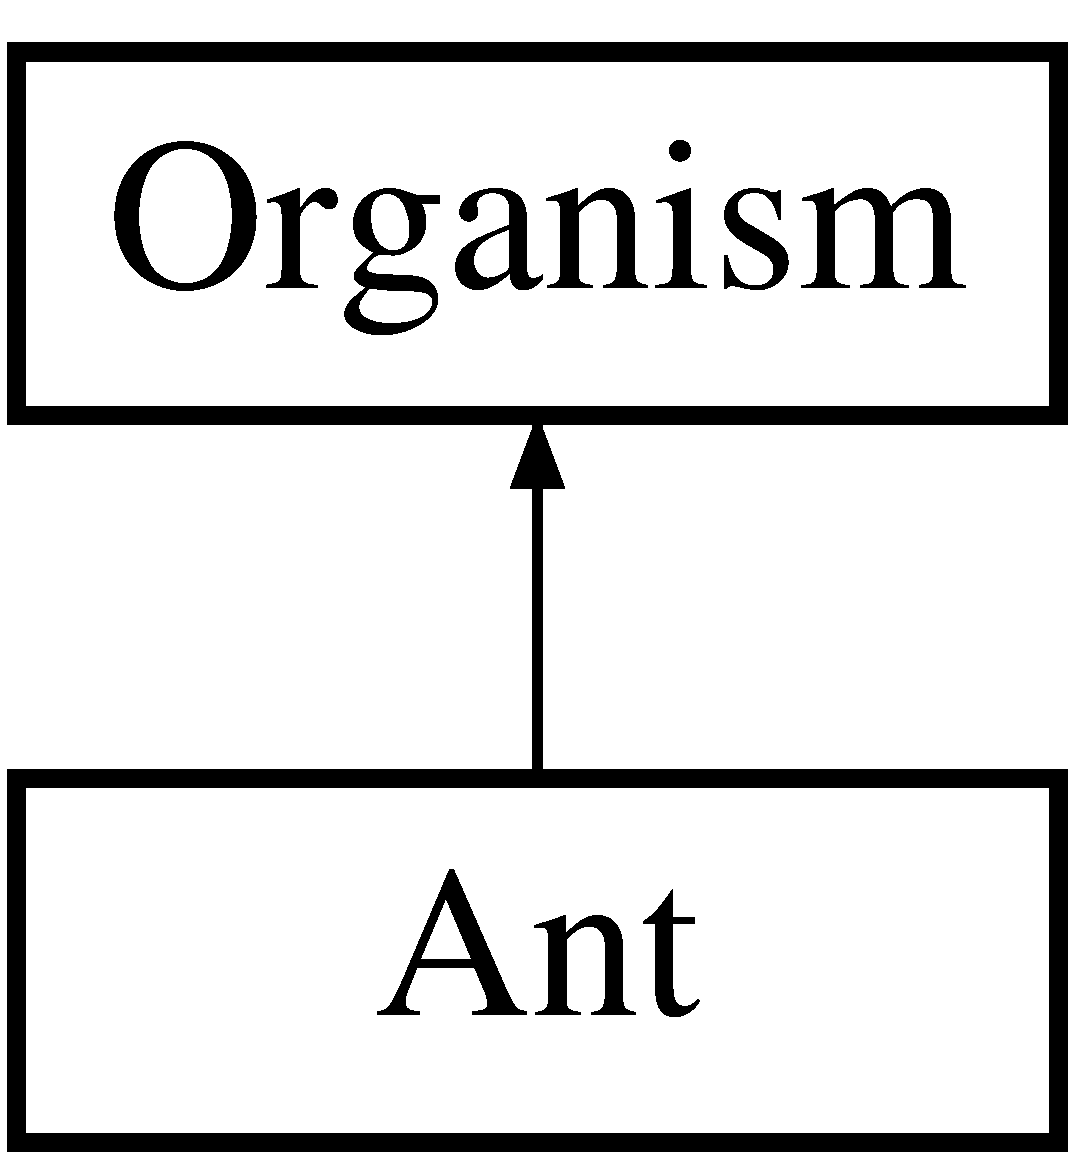
\includegraphics[height=2.000000cm]{classAnt}
\end{center}
\end{figure}
\subsection*{Public Member Functions}
\begin{DoxyCompactItemize}
\item 
\textbf{ Ant} ()
\item 
\textbf{ Ant} (int r, int c, \textbf{ Grid} $\ast$ptr)
\item 
bool \textbf{ move} ()
\item 
bool \textbf{ breed} ()
\item 
bool \textbf{ step} ()
\item 
bool \textbf{ increm} ()
\item 
bool \textbf{ set\+Breed\+Cnt} (int i)
\item 
bool \textbf{ set\+Row\+And\+Col} (int i, int j)
\item 
bool \textbf{ set\+Grid\+Ptr} (\textbf{ Grid} $\ast$a)
\item 
struct \textbf{ Organism\+::\+Coordinates} \textbf{ get\+Rand\+Cell} (int \textbf{ row}, int \textbf{ col}, \textbf{ Grid} $\ast$\textbf{ g})
\item 
\textbf{ $\sim$\+Ant} ()
\end{DoxyCompactItemize}
\subsection*{Private Attributes}
\begin{DoxyCompactItemize}
\item 
int \textbf{ row} = 0
\item 
int \textbf{ col} = 0
\item 
int \textbf{ breed\+Cnt} = 0
\item 
\textbf{ Grid} $\ast$ \textbf{ g} = nullptr
\end{DoxyCompactItemize}


\subsection{Constructor \& Destructor Documentation}
\mbox{\label{classAnt_ad6c1a8f70419877f7a3e2c9c557f913d}} 
\index{Ant@{Ant}!Ant@{Ant}}
\index{Ant@{Ant}!Ant@{Ant}}
\subsubsection{Ant()\hspace{0.1cm}{\footnotesize\ttfamily [1/2]}}
{\footnotesize\ttfamily Ant\+::\+Ant (\begin{DoxyParamCaption}{ }\end{DoxyParamCaption})}

\doxyref{Ant\+::\+Ant()}{p.}{classAnt_ad6c1a8f70419877f7a3e2c9c557f913d} is the basic constructor for the ant class 
\begin{DoxyParams}{Parameters}
{\em none} & \\
\hline
\end{DoxyParams}
\begin{DoxyReturn}{Returns}
none 
\end{DoxyReturn}


Referenced by breed(), and Tests2\+::organism\+Rand\+Cell\+Test().

\mbox{\label{classAnt_a234f9425fb253250f230cfcca9eb4e9f}} 
\index{Ant@{Ant}!Ant@{Ant}}
\index{Ant@{Ant}!Ant@{Ant}}
\subsubsection{Ant()\hspace{0.1cm}{\footnotesize\ttfamily [2/2]}}
{\footnotesize\ttfamily Ant\+::\+Ant (\begin{DoxyParamCaption}\item[{int}]{r,  }\item[{int}]{c,  }\item[{\textbf{ Grid} $\ast$}]{ptr }\end{DoxyParamCaption})}

\doxyref{Ant\+::\+Ant()}{p.}{classAnt_ad6c1a8f70419877f7a3e2c9c557f913d} is another constructor for the ant class, placing the ant object at the location on the grid specified by the row and column parameters 
\begin{DoxyParams}{Parameters}
{\em int} & r, the row where the ant will be constructed \\
\hline
{\em int} & c, the column where the ant will be constructed \\
\hline
{\em int} & life, the amount of ticks the ant object has been alive on the board \\
\hline
\end{DoxyParams}
\begin{DoxyReturn}{Returns}
none 
\end{DoxyReturn}


References col, g, and row.

\mbox{\label{classAnt_a33ca6bd592236726a18a2159908e4116}} 
\index{Ant@{Ant}!````~Ant@{$\sim$\+Ant}}
\index{````~Ant@{$\sim$\+Ant}!Ant@{Ant}}
\subsubsection{$\sim$\+Ant()}
{\footnotesize\ttfamily Ant\+::$\sim$\+Ant (\begin{DoxyParamCaption}{ }\end{DoxyParamCaption})}

\doxyref{Ant\+::$\sim$\+Ant}{p.}{classAnt_a33ca6bd592236726a18a2159908e4116} is a destructor for the ant class 
\begin{DoxyParams}{Parameters}
{\em none} & indicating that a ant object has died \\
\hline
\end{DoxyParams}


References col, empty, g, row, Grid\+::set\+Cell\+Occupant(), Grid\+::set\+Cell\+Organism(), and set\+Grid\+Ptr().



Referenced by Tests2\+::ants\+Breed\+Test(), Tests2\+::ants\+Die\+Test(), Tests2\+::ants\+Move\+Test(), Doodlebug\+::eat(), Tests2\+::make\+Ants\+Test(), and Tests2\+::\+Organism\+Test().



\subsection{Member Function Documentation}
\mbox{\label{classAnt_a13f4550006f7d3626ba4c0af215e06b6}} 
\index{Ant@{Ant}!breed@{breed}}
\index{breed@{breed}!Ant@{Ant}}
\subsubsection{breed()}
{\footnotesize\ttfamily bool Ant\+::breed (\begin{DoxyParamCaption}{ }\end{DoxyParamCaption})\hspace{0.3cm}{\ttfamily [virtual]}}

\doxyref{Ant\+::breed()}{p.}{classAnt_a13f4550006f7d3626ba4c0af215e06b6} should check the cells around the ant object and if another ant in is a neighboring cell, then they will produce a new ant object in a free space 
\begin{DoxyParams}{Parameters}
{\em Grid$\ast$} & g grid we are on \\
\hline
\end{DoxyParams}
\begin{DoxyReturn}{Returns}
status true if ant breed 
\end{DoxyReturn}


Implements \textbf{ Organism} \doxyref{}{p.}{classOrganism_a0336595710b1b4e7996852596d8be619}.



References ant, Ant(), Organism\+::\+Coordinates\+::cell\+Col, Organism\+::\+Coordinates\+::cell\+Row, col, g, Grid\+::get\+Num\+Ant(), get\+Rand\+Cell(), increm(), row, set\+Breed\+Cnt(), Grid\+::set\+Cell\+Occupant(), Grid\+::set\+Cell\+Organism(), and Grid\+::set\+Num\+Ant().



Referenced by Tests2\+::ants\+Breed\+Test(), and step().

\mbox{\label{classAnt_a3889cd201fe6a10eabd47b90a28045ce}} 
\index{Ant@{Ant}!get\+Rand\+Cell@{get\+Rand\+Cell}}
\index{get\+Rand\+Cell@{get\+Rand\+Cell}!Ant@{Ant}}
\subsubsection{get\+Rand\+Cell()}
{\footnotesize\ttfamily struct \textbf{ Ant\+::\+Coordinates} Ant\+::get\+Rand\+Cell (\begin{DoxyParamCaption}\item[{int}]{row,  }\item[{int}]{col,  }\item[{\textbf{ Grid} $\ast$}]{g }\end{DoxyParamCaption})\hspace{0.3cm}{\ttfamily [virtual]}}

Ant\+::\+Get\+Rand\+Cell takes an array of pointers to cells and returns a pseudo-\/random cell that is a neighbor of the input cell (row and cel).. 
\begin{DoxyParams}{Parameters}
{\em int} & row, the row that this cell is on \\
\hline
{\em int} & col, the column that this cell is on \\
\hline
{\em \doxyref{Grid}{p.}{classGrid}} & g is the grid of cells \\
\hline
\end{DoxyParams}
\begin{DoxyReturn}{Returns}
output, a struct Coordinates which represents the row and column of the randomly chosen cell 
\end{DoxyReturn}


Reimplemented from \textbf{ Organism} \doxyref{}{p.}{classOrganism_a52ff86e2ef1b525ffc5a473cfee8080e}.



References Organism\+::\+Coordinates\+::cell\+Col, Organism\+::\+Coordinates\+::cell\+Row, col, empty, g, Grid\+::get\+Cell\+Occupant(), Grid\+::get\+Num\+Cells(), Organism\+::num\+Poss\+Cells(), and row.



Referenced by breed(), move(), and Tests2\+::organism\+Rand\+Cell\+Test().

\mbox{\label{classAnt_a8b4e65af7752399808703ca6cc87a601}} 
\index{Ant@{Ant}!increm@{increm}}
\index{increm@{increm}!Ant@{Ant}}
\subsubsection{increm()}
{\footnotesize\ttfamily bool Ant\+::increm (\begin{DoxyParamCaption}{ }\end{DoxyParamCaption})}

\doxyref{Ant\+::increm()}{p.}{classAnt_a8b4e65af7752399808703ca6cc87a601}-\/ used to increment the breed counters inside of the ant. 
\begin{DoxyParams}{Parameters}
{\em none} & \\
\hline
\end{DoxyParams}
\begin{DoxyReturn}{Returns}
bool result true if the function ran properly 
\end{DoxyReturn}


References breed\+Cnt.



Referenced by breed(), and step().

\mbox{\label{classAnt_a4aa0576c34e25ca4df23f90a3caef0f5}} 
\index{Ant@{Ant}!move@{move}}
\index{move@{move}!Ant@{Ant}}
\subsubsection{move()}
{\footnotesize\ttfamily bool Ant\+::move (\begin{DoxyParamCaption}{ }\end{DoxyParamCaption})\hspace{0.3cm}{\ttfamily [virtual]}}

\doxyref{Ant\+::move()}{p.}{classAnt_a4aa0576c34e25ca4df23f90a3caef0f5} should move an ant object to a neighboring cell 
\begin{DoxyParams}{Parameters}
{\em none} & \\
\hline
\end{DoxyParams}
\begin{DoxyReturn}{Returns}
status, true if the ant object moved 
\end{DoxyReturn}


Implements \textbf{ Organism} \doxyref{}{p.}{classOrganism_a9b6a5dadbe12711fa252bbfbfb988545}.



References ant, Organism\+::\+Coordinates\+::cell\+Col, Organism\+::\+Coordinates\+::cell\+Row, col, empty, g, Grid\+::get\+Cell\+Organism(), get\+Rand\+Cell(), row, Grid\+::set\+Cell\+Occupant(), Grid\+::set\+Cell\+Organism(), and set\+Row\+And\+Col().



Referenced by Tests2\+::ants\+Move\+Test(), and step().

\mbox{\label{classAnt_a9e07799223c8a57c436b2982299b9c22}} 
\index{Ant@{Ant}!set\+Breed\+Cnt@{set\+Breed\+Cnt}}
\index{set\+Breed\+Cnt@{set\+Breed\+Cnt}!Ant@{Ant}}
\subsubsection{set\+Breed\+Cnt()}
{\footnotesize\ttfamily bool Ant\+::set\+Breed\+Cnt (\begin{DoxyParamCaption}\item[{int}]{i }\end{DoxyParamCaption})}

\doxyref{Ant\+::set\+Breed\+Cnt}{p.}{classAnt_a9e07799223c8a57c436b2982299b9c22} Sets the Breed Count inside of the ant 
\begin{DoxyParams}{Parameters}
{\em int} & i the new count to i \\
\hline
{\em bool} & result true if the function worked \\
\hline
\end{DoxyParams}


References breed\+Cnt.



Referenced by breed().

\mbox{\label{classAnt_a60bcbfb2c76e60dd37434acf797a254e}} 
\index{Ant@{Ant}!set\+Grid\+Ptr@{set\+Grid\+Ptr}}
\index{set\+Grid\+Ptr@{set\+Grid\+Ptr}!Ant@{Ant}}
\subsubsection{set\+Grid\+Ptr()}
{\footnotesize\ttfamily bool Ant\+::set\+Grid\+Ptr (\begin{DoxyParamCaption}\item[{\textbf{ Grid} $\ast$}]{a }\end{DoxyParamCaption})}

\doxyref{Ant\+::set\+Grid\+Ptr}{p.}{classAnt_a60bcbfb2c76e60dd37434acf797a254e} Sets the grid pointer for the ant 
\begin{DoxyParams}{Parameters}
{\em none} & \\
\hline
\end{DoxyParams}
\begin{DoxyReturn}{Returns}
bool true if the function worked 
\end{DoxyReturn}


References g.



Referenced by $\sim$\+Ant().

\mbox{\label{classAnt_adb3266abdb4fbf6c56edd8c7fca768dc}} 
\index{Ant@{Ant}!set\+Row\+And\+Col@{set\+Row\+And\+Col}}
\index{set\+Row\+And\+Col@{set\+Row\+And\+Col}!Ant@{Ant}}
\subsubsection{set\+Row\+And\+Col()}
{\footnotesize\ttfamily bool Ant\+::set\+Row\+And\+Col (\begin{DoxyParamCaption}\item[{int}]{i,  }\item[{int}]{j }\end{DoxyParamCaption})}

\doxyref{Ant\+::set\+Row\+And\+Col}{p.}{classAnt_adb3266abdb4fbf6c56edd8c7fca768dc} set the row and column of the \doxyref{Ant}{p.}{classAnt} 
\begin{DoxyParams}{Parameters}
{\em int} & i the new row \\
\hline
{\em int} & j the new column \\
\hline
{\em bool} & result true if function worked \\
\hline
\end{DoxyParams}


References col, and row.



Referenced by move().

\mbox{\label{classAnt_ae7bb9517e9090218401d83fa2858561a}} 
\index{Ant@{Ant}!step@{step}}
\index{step@{step}!Ant@{Ant}}
\subsubsection{step()}
{\footnotesize\ttfamily bool Ant\+::step (\begin{DoxyParamCaption}{ }\end{DoxyParamCaption})\hspace{0.3cm}{\ttfamily [virtual]}}

Ant\+::\+Step() performs a move and breed if the conditions for moving and breeding are met. 
\begin{DoxyParams}{Parameters}
{\em none} & \\
\hline
\end{DoxyParams}
\begin{DoxyReturn}{Returns}
bool if the step worked 
\end{DoxyReturn}


Implements \textbf{ Organism} \doxyref{}{p.}{classOrganism_ae889d5671066bccdfbc15c7f16eab20e}.



References breed(), breed\+Cnt, col, g, Grid\+::get\+Num\+Ant(), increm(), move(), Organism\+::num\+Poss\+Cells(), row, and Grid\+::set\+Num\+Ant().



\subsection{Field Documentation}
\mbox{\label{classAnt_ada40f54e63324c09a57961fb726149da}} 
\index{Ant@{Ant}!breed\+Cnt@{breed\+Cnt}}
\index{breed\+Cnt@{breed\+Cnt}!Ant@{Ant}}
\subsubsection{breed\+Cnt}
{\footnotesize\ttfamily int Ant\+::breed\+Cnt = 0\hspace{0.3cm}{\ttfamily [private]}}



Referenced by increm(), set\+Breed\+Cnt(), and step().

\mbox{\label{classAnt_afe21bedec87ea26e3db74857960a78c6}} 
\index{Ant@{Ant}!col@{col}}
\index{col@{col}!Ant@{Ant}}
\subsubsection{col}
{\footnotesize\ttfamily int Ant\+::col = 0\hspace{0.3cm}{\ttfamily [private]}}



Referenced by Ant(), breed(), get\+Rand\+Cell(), move(), set\+Row\+And\+Col(), step(), and $\sim$\+Ant().

\mbox{\label{classAnt_a60e006b25b0905b95ed3a636febdba2e}} 
\index{Ant@{Ant}!g@{g}}
\index{g@{g}!Ant@{Ant}}
\subsubsection{g}
{\footnotesize\ttfamily \textbf{ Grid}$\ast$ Ant\+::g = nullptr\hspace{0.3cm}{\ttfamily [private]}}



Referenced by Ant(), breed(), get\+Rand\+Cell(), move(), set\+Grid\+Ptr(), step(), and $\sim$\+Ant().

\mbox{\label{classAnt_abf712c4a02e999938c7d79557a8fc24b}} 
\index{Ant@{Ant}!row@{row}}
\index{row@{row}!Ant@{Ant}}
\subsubsection{row}
{\footnotesize\ttfamily int Ant\+::row = 0\hspace{0.3cm}{\ttfamily [private]}}



Referenced by Ant(), breed(), get\+Rand\+Cell(), move(), set\+Row\+And\+Col(), step(), and $\sim$\+Ant().



The documentation for this class was generated from the following files\+:\begin{DoxyCompactItemize}
\item 
\textbf{ Ant.\+h}\item 
\textbf{ Ant.\+cpp}\end{DoxyCompactItemize}

\section{Cell Class Reference}
\label{classCell}\index{Cell@{Cell}}


{\ttfamily \#include $<$Cell.\+h$>$}

\subsection*{Public Member Functions}
\begin{DoxyCompactItemize}
\item 
\textbf{ Cell} ()
\item 
bool \textbf{ set\+Occupant} (\textbf{ occupation\+Status} g)
\item 
\textbf{ occupation\+Status} \textbf{ get\+Occupant} ()
\item 
bool \textbf{ set\+Organism} (\textbf{ Organism} $\ast$o)
\item 
\textbf{ Organism} $\ast$ \textbf{ get\+Organism} ()
\item 
virtual \textbf{ $\sim$\+Cell} ()
\end{DoxyCompactItemize}
\subsection*{Private Attributes}
\begin{DoxyCompactItemize}
\item 
\textbf{ occupation\+Status} \textbf{ guest} = \textbf{ empty}
\item 
\textbf{ Organism} $\ast$ \textbf{ p} = nullptr
\end{DoxyCompactItemize}


\subsection{Constructor \& Destructor Documentation}
\mbox{\label{classCell_a394510643e8664cf12b5efaf5cb99f71}} 
\index{Cell@{Cell}!Cell@{Cell}}
\index{Cell@{Cell}!Cell@{Cell}}
\subsubsection{Cell()}
{\footnotesize\ttfamily Cell\+::\+Cell (\begin{DoxyParamCaption}{ }\end{DoxyParamCaption})}

\doxyref{Cell\+::\+Cell()}{p.}{classCell_a394510643e8664cf12b5efaf5cb99f71} is a constructor of a cell 
\begin{DoxyParams}{Parameters}
{\em none} & \\
\hline
\end{DoxyParams}
\begin{DoxyReturn}{Returns}
none 
\end{DoxyReturn}
\mbox{\label{classCell_a9fa559f7a28e2b4336c6879ca09304d8}} 
\index{Cell@{Cell}!````~Cell@{$\sim$\+Cell}}
\index{````~Cell@{$\sim$\+Cell}!Cell@{Cell}}
\subsubsection{$\sim$\+Cell()}
{\footnotesize\ttfamily Cell\+::$\sim$\+Cell (\begin{DoxyParamCaption}{ }\end{DoxyParamCaption})\hspace{0.3cm}{\ttfamily [virtual]}}

\doxyref{Cell\+::$\sim$\+Cell}{p.}{classCell_a9fa559f7a28e2b4336c6879ca09304d8} is the destructor for a cell  none \begin{DoxyReturn}{Returns}
none 
\end{DoxyReturn}


Referenced by Grid\+::$\sim$\+Grid().



\subsection{Member Function Documentation}
\mbox{\label{classCell_a7dcb8bc75a2e2591b3fd52b5f7c28ab1}} 
\index{Cell@{Cell}!get\+Occupant@{get\+Occupant}}
\index{get\+Occupant@{get\+Occupant}!Cell@{Cell}}
\subsubsection{get\+Occupant()}
{\footnotesize\ttfamily \textbf{ occupation\+Status} Cell\+::get\+Occupant (\begin{DoxyParamCaption}{ }\end{DoxyParamCaption})}

Cell\+::qet\+Occupant gets the occupant\+Status of the cell 
\begin{DoxyParams}{Parameters}
{\em none} & \\
\hline
\end{DoxyParams}
\begin{DoxyReturn}{Returns}
the occupation\+Status of a cell which is an enumeration that can be empty, ant or doodlebug and represents what organism is in the cell 
\end{DoxyReturn}


References guest.



Referenced by Grid\+::get\+Cell\+Occupant().

\mbox{\label{classCell_acea25bbe9675482cf4ad8f3596c78300}} 
\index{Cell@{Cell}!get\+Organism@{get\+Organism}}
\index{get\+Organism@{get\+Organism}!Cell@{Cell}}
\subsubsection{get\+Organism()}
{\footnotesize\ttfamily \textbf{ Organism} $\ast$ Cell\+::get\+Organism (\begin{DoxyParamCaption}{ }\end{DoxyParamCaption})}

\doxyref{Cell\+::get\+Organism}{p.}{classCell_acea25bbe9675482cf4ad8f3596c78300} gets the field p which is the pointer to the organism that is currently in the cell 
\begin{DoxyParams}{Parameters}
{\em none} & \\
\hline
\end{DoxyParams}
\begin{DoxyReturn}{Returns}
Organism$\ast$ p, The pointer to the organism in the current cell 
\end{DoxyReturn}


References p.



Referenced by Grid\+::get\+Cell\+Organism().

\mbox{\label{classCell_a2346933316b45d87264d50e563c2f895}} 
\index{Cell@{Cell}!set\+Occupant@{set\+Occupant}}
\index{set\+Occupant@{set\+Occupant}!Cell@{Cell}}
\subsubsection{set\+Occupant()}
{\footnotesize\ttfamily bool Cell\+::set\+Occupant (\begin{DoxyParamCaption}\item[{\textbf{ occupation\+Status}}]{g }\end{DoxyParamCaption})}

\doxyref{Cell\+::set\+Occupant}{p.}{classCell_a2346933316b45d87264d50e563c2f895} sets the occupation\+Status of cell 
\begin{DoxyParams}{Parameters}
{\em occupation\+Status} & g, is an enumeration that can be empty, ant or doodlebug and represents what organism is in the cell \\
\hline
\end{DoxyParams}
\begin{DoxyReturn}{Returns}
bool result of if this worked 
\end{DoxyReturn}


References Production\+::g, and guest.



Referenced by Grid\+::set\+Cell\+Occupant().

\mbox{\label{classCell_a4e3175ebd6973bb590d38e9325002f4f}} 
\index{Cell@{Cell}!set\+Organism@{set\+Organism}}
\index{set\+Organism@{set\+Organism}!Cell@{Cell}}
\subsubsection{set\+Organism()}
{\footnotesize\ttfamily bool Cell\+::set\+Organism (\begin{DoxyParamCaption}\item[{\textbf{ Organism} $\ast$}]{o }\end{DoxyParamCaption})}

\doxyref{Cell\+::set\+Organism}{p.}{classCell_a4e3175ebd6973bb590d38e9325002f4f} sets the field p which is the pointer to the organism that is currently in the cell 
\begin{DoxyParams}{Parameters}
{\em Organism$\ast$} & o, The pointer to the organism that you want to put in the current cell \\
\hline
\end{DoxyParams}
\begin{DoxyReturn}{Returns}
bool if the function was successful 
\end{DoxyReturn}


References p.



Referenced by Grid\+::set\+Cell\+Organism().



\subsection{Field Documentation}
\mbox{\label{classCell_aafc273a5125cf29742a8df6f5a5a881c}} 
\index{Cell@{Cell}!guest@{guest}}
\index{guest@{guest}!Cell@{Cell}}
\subsubsection{guest}
{\footnotesize\ttfamily \textbf{ occupation\+Status} Cell\+::guest = \textbf{ empty}\hspace{0.3cm}{\ttfamily [private]}}



Referenced by get\+Occupant(), and set\+Occupant().

\mbox{\label{classCell_a8ce33921a2a925d8ad057b08c8fc0671}} 
\index{Cell@{Cell}!p@{p}}
\index{p@{p}!Cell@{Cell}}
\subsubsection{p}
{\footnotesize\ttfamily \textbf{ Organism}$\ast$ Cell\+::p = nullptr\hspace{0.3cm}{\ttfamily [private]}}



Referenced by get\+Organism(), and set\+Organism().



The documentation for this class was generated from the following files\+:\begin{DoxyCompactItemize}
\item 
\textbf{ Cell.\+h}\item 
\textbf{ Cell.\+cpp}\end{DoxyCompactItemize}

\section{Organism\+:\+:Coordinates Struct Reference}
\label{structOrganism_1_1Coordinates}\index{Organism\+::\+Coordinates@{Organism\+::\+Coordinates}}


{\ttfamily \#include $<$Organism.\+h$>$}

\subsection*{Data Fields}
\begin{DoxyCompactItemize}
\item 
int \textbf{ cell\+Row}
\item 
int \textbf{ cell\+Col}
\end{DoxyCompactItemize}


\subsection{Field Documentation}
\mbox{\label{structOrganism_1_1Coordinates_af549776fba430bdffc4e5db3a30bc7fb}} 
\index{Organism\+::\+Coordinates@{Organism\+::\+Coordinates}!cell\+Col@{cell\+Col}}
\index{cell\+Col@{cell\+Col}!Organism\+::\+Coordinates@{Organism\+::\+Coordinates}}
\subsubsection{cell\+Col}
{\footnotesize\ttfamily int Organism\+::\+Coordinates\+::cell\+Col}



Referenced by Ant\+::breed(), Doodlebug\+::breed\+Doodle(), Doodlebug\+::eat(), Organism\+::get\+Rand\+Cell(), Ant\+::get\+Rand\+Cell(), Doodlebug\+::get\+Rand\+Cell(), Ant\+::move(), Doodlebug\+::move(), and Tests2\+::organism\+Rand\+Cell\+Test().

\mbox{\label{structOrganism_1_1Coordinates_a9bb1c31af6af3468294851c581b01e83}} 
\index{Organism\+::\+Coordinates@{Organism\+::\+Coordinates}!cell\+Row@{cell\+Row}}
\index{cell\+Row@{cell\+Row}!Organism\+::\+Coordinates@{Organism\+::\+Coordinates}}
\subsubsection{cell\+Row}
{\footnotesize\ttfamily int Organism\+::\+Coordinates\+::cell\+Row}



Referenced by Ant\+::breed(), Doodlebug\+::breed\+Doodle(), Doodlebug\+::eat(), Organism\+::get\+Rand\+Cell(), Ant\+::get\+Rand\+Cell(), Doodlebug\+::get\+Rand\+Cell(), Ant\+::move(), Doodlebug\+::move(), and Tests2\+::organism\+Rand\+Cell\+Test().



The documentation for this struct was generated from the following file\+:\begin{DoxyCompactItemize}
\item 
\textbf{ Organism.\+h}\end{DoxyCompactItemize}

\section{Doodlebug Class Reference}
\label{classDoodlebug}\index{Doodlebug@{Doodlebug}}


{\ttfamily \#include $<$Doodlebug.\+h$>$}

Inheritance diagram for Doodlebug\+:\begin{figure}[H]
\begin{center}
\leavevmode
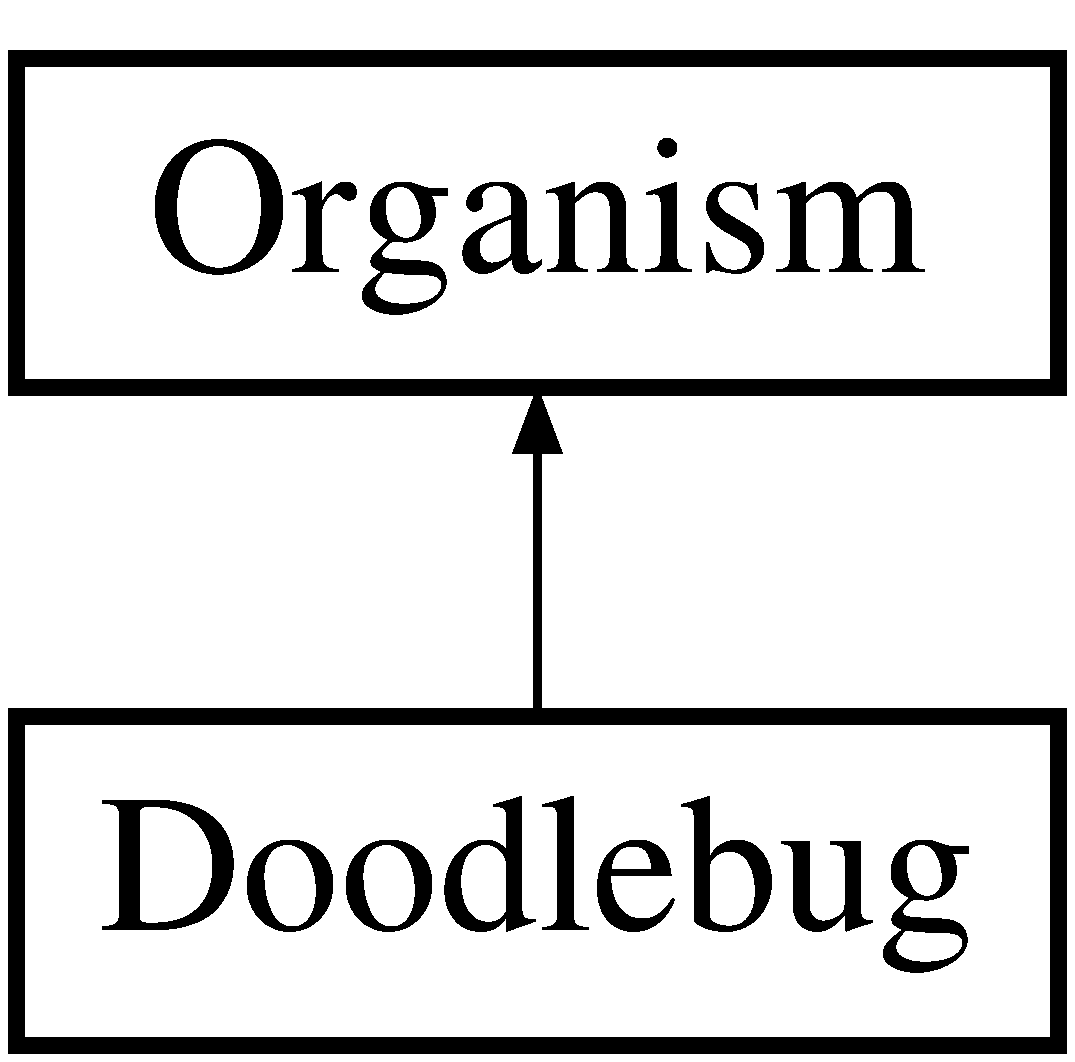
\includegraphics[height=2.000000cm]{classDoodlebug}
\end{center}
\end{figure}
\subsection*{Public Member Functions}
\begin{DoxyCompactItemize}
\item 
\textbf{ Doodlebug} ()
\item 
\textbf{ Doodlebug} (int r, int c, \textbf{ Grid} $\ast$ptr)
\item 
bool \textbf{ move} ()
\item 
bool \textbf{ breed} ()
\item 
bool \textbf{ breed\+Doodle} ()
\item 
bool \textbf{ eat} ()
\item 
int \textbf{ get\+Starve\+Cnt} ()
\item 
bool \textbf{ set\+Starve\+Cnt} (int s)
\item 
\textbf{ $\sim$\+Doodlebug} ()
\item 
bool \textbf{ step} ()
\item 
bool \textbf{ increm} ()
\item 
bool \textbf{ set\+Breed\+Cnt} (int i)
\item 
int \textbf{ num\+Poss\+Cells} (int \textbf{ row}, int \textbf{ col}, \textbf{ Grid} $\ast$\textbf{ g})
\item 
bool \textbf{ set\+Grid\+Ptr} (\textbf{ Grid} $\ast$a)
\item 
bool \textbf{ set\+Row\+And\+Col} (int i, int j)
\item 
struct \textbf{ Organism\+::\+Coordinates} \textbf{ get\+Rand\+Cell} (int \textbf{ row}, int \textbf{ col}, \textbf{ Grid} $\ast$\textbf{ g})
\end{DoxyCompactItemize}
\subsection*{Private Attributes}
\begin{DoxyCompactItemize}
\item 
int \textbf{ row} = 0
\item 
int \textbf{ col} = 0
\item 
int \textbf{ starve\+Cnt} = 0
\item 
int \textbf{ breed\+Cnt} = 0
\item 
\textbf{ Grid} $\ast$ \textbf{ g} = nullptr
\end{DoxyCompactItemize}


\subsection{Constructor \& Destructor Documentation}
\mbox{\label{classDoodlebug_afb2796ea39a6ffa13d4f54ac68dd52fc}} 
\index{Doodlebug@{Doodlebug}!Doodlebug@{Doodlebug}}
\index{Doodlebug@{Doodlebug}!Doodlebug@{Doodlebug}}
\subsubsection{Doodlebug()\hspace{0.1cm}{\footnotesize\ttfamily [1/2]}}
{\footnotesize\ttfamily Doodlebug\+::\+Doodlebug (\begin{DoxyParamCaption}{ }\end{DoxyParamCaption})}

\doxyref{Doodlebug\+::\+Doodlebug()}{p.}{classDoodlebug_afb2796ea39a6ffa13d4f54ac68dd52fc} Default Constructor 
\begin{DoxyParams}{Parameters}
{\em false} & is set for the organism input to tell the organism that it is not an ant \\
\hline
\end{DoxyParams}
\begin{DoxyReturn}{Returns}
none 
\end{DoxyReturn}


Referenced by breed\+Doodle().

\mbox{\label{classDoodlebug_a30b896467b713684c59ee97767c97f50}} 
\index{Doodlebug@{Doodlebug}!Doodlebug@{Doodlebug}}
\index{Doodlebug@{Doodlebug}!Doodlebug@{Doodlebug}}
\subsubsection{Doodlebug()\hspace{0.1cm}{\footnotesize\ttfamily [2/2]}}
{\footnotesize\ttfamily Doodlebug\+::\+Doodlebug (\begin{DoxyParamCaption}\item[{int}]{r,  }\item[{int}]{c,  }\item[{\textbf{ Grid} $\ast$}]{ptr }\end{DoxyParamCaption})}

\doxyref{Doodlebug\+::\+Doodlebug()}{p.}{classDoodlebug_afb2796ea39a6ffa13d4f54ac68dd52fc}\+:\doxyref{Organism()}{p.}{classOrganism_aeb16ee24b64839584b4862384d0b53fe} Constructor 
\begin{DoxyParams}{Parameters}
{\em int} & r, The row the doodlebug should be constructed on \\
\hline
{\em int} & c, The col the doodlebug should be constructed on \\
\hline
{\em \doxyref{Grid}{p.}{classGrid}} & $\ast$ ptr, The pointer to the grid the doodlebug is geing created on \\
\hline
{\em false} & is set for the organism input to tell the organism that it is not an ant \doxyref{Doodlebug}{p.}{classDoodlebug} will have a Starve Counter and a Breed Counter it will also have a row and col for its location \\
\hline
\end{DoxyParams}
\begin{DoxyReturn}{Returns}
none 
\end{DoxyReturn}


References col, g, and row.

\mbox{\label{classDoodlebug_ac318cc9acbd9a3af52348a236070d891}} 
\index{Doodlebug@{Doodlebug}!````~Doodlebug@{$\sim$\+Doodlebug}}
\index{````~Doodlebug@{$\sim$\+Doodlebug}!Doodlebug@{Doodlebug}}
\subsubsection{$\sim$\+Doodlebug()}
{\footnotesize\ttfamily Doodlebug\+::$\sim$\+Doodlebug (\begin{DoxyParamCaption}{ }\end{DoxyParamCaption})}

\doxyref{Doodlebug\+::$\sim$\+Doodlebug()}{p.}{classDoodlebug_ac318cc9acbd9a3af52348a236070d891} Destructor, used to remove a pointer to a doodlebug 
\begin{DoxyParams}{Parameters}
{\em none} & \\
\hline
\end{DoxyParams}
\begin{DoxyReturn}{Returns}
none 
\end{DoxyReturn}


References col, empty, g, row, Grid\+::set\+Cell\+Occupant(), Grid\+::set\+Cell\+Organism(), and set\+Grid\+Ptr().



Referenced by Tests2\+::ants\+Move\+Test(), Tests2\+::doodle\+Breed\+Test(), Tests2\+::doodle\+Dietest(), Tests2\+::doodle\+Eat\+Test(), Tests2\+::doodle\+Move\+Test(), Tests2\+::make\+Doodles\+Test(), and step().



\subsection{Member Function Documentation}
\mbox{\label{classDoodlebug_af88c6c6331094b012597ac2c688018d7}} 
\index{Doodlebug@{Doodlebug}!breed@{breed}}
\index{breed@{breed}!Doodlebug@{Doodlebug}}
\subsubsection{breed()}
{\footnotesize\ttfamily bool Doodlebug\+::breed (\begin{DoxyParamCaption}{ }\end{DoxyParamCaption})\hspace{0.3cm}{\ttfamily [virtual]}}



Implements \textbf{ Organism} \doxyref{}{p.}{classOrganism_a0336595710b1b4e7996852596d8be619}.

\mbox{\label{classDoodlebug_a43bd72741f99da0044319d379475a2fb}} 
\index{Doodlebug@{Doodlebug}!breed\+Doodle@{breed\+Doodle}}
\index{breed\+Doodle@{breed\+Doodle}!Doodlebug@{Doodlebug}}
\subsubsection{breed\+Doodle()}
{\footnotesize\ttfamily bool Doodlebug\+::breed\+Doodle (\begin{DoxyParamCaption}{ }\end{DoxyParamCaption})}

\doxyref{Doodlebug\+::breed()}{p.}{classDoodlebug_af88c6c6331094b012597ac2c688018d7}, finds a random unoccupied neighboring cell and creates a new doodlebug inside it. Breeding does N\+OT take precidence over death 
\begin{DoxyParams}{Parameters}
{\em none} & \\
\hline
\end{DoxyParams}
\begin{DoxyReturn}{Returns}
bool returns true if the bug was able to breed 
\end{DoxyReturn}


References Organism\+::\+Coordinates\+::cell\+Col, Organism\+::\+Coordinates\+::cell\+Row, col, doodlebug, Doodlebug(), g, Grid\+::get\+Num\+Doodle(), Organism\+::get\+Rand\+Cell(), row, set\+Breed\+Cnt(), Grid\+::set\+Cell\+Occupant(), Grid\+::set\+Cell\+Organism(), and Grid\+::set\+Num\+Doodle().



Referenced by Tests2\+::doodle\+Breed\+Test(), and step().

\mbox{\label{classDoodlebug_a6c35a8891356525e644330339690ccc6}} 
\index{Doodlebug@{Doodlebug}!eat@{eat}}
\index{eat@{eat}!Doodlebug@{Doodlebug}}
\subsubsection{eat()}
{\footnotesize\ttfamily bool Doodlebug\+::eat (\begin{DoxyParamCaption}{ }\end{DoxyParamCaption})}

\doxyref{Doodlebug\+::eat()}{p.}{classDoodlebug_a6c35a8891356525e644330339690ccc6} finds a neighboring cell that contains an ant and resets the doodlebug\textquotesingle{}s starve counter, also destructs the ant Eating takes precedence over the majority of other actions 
\begin{DoxyParams}{Parameters}
{\em none} & \\
\hline
\end{DoxyParams}
\begin{DoxyReturn}{Returns}
bool returns true if the bug was able to eat 
\end{DoxyReturn}


References Organism\+::\+Coordinates\+::cell\+Col, Organism\+::\+Coordinates\+::cell\+Row, col, doodlebug, empty, g, Grid\+::get\+Cell\+Organism(), Grid\+::get\+Num\+Ant(), get\+Rand\+Cell(), row, Grid\+::set\+Cell\+Occupant(), Grid\+::set\+Cell\+Organism(), Grid\+::set\+Num\+Ant(), set\+Row\+And\+Col(), set\+Starve\+Cnt(), and Ant\+::$\sim$\+Ant().



Referenced by Tests2\+::doodle\+Eat\+Test(), and step().

\mbox{\label{classDoodlebug_a4e8a8ced92f0624cb6ca8e1103f5c435}} 
\index{Doodlebug@{Doodlebug}!get\+Rand\+Cell@{get\+Rand\+Cell}}
\index{get\+Rand\+Cell@{get\+Rand\+Cell}!Doodlebug@{Doodlebug}}
\subsubsection{get\+Rand\+Cell()}
{\footnotesize\ttfamily struct \textbf{ Doodlebug\+::\+Coordinates} Doodlebug\+::get\+Rand\+Cell (\begin{DoxyParamCaption}\item[{int}]{row,  }\item[{int}]{col,  }\item[{\textbf{ Grid} $\ast$}]{g }\end{DoxyParamCaption})\hspace{0.3cm}{\ttfamily [virtual]}}

Get\+Rand\+Cell takes an array of pointers to cells and returns a pseudo-\/random cell that neighbors the input row column pair. 
\begin{DoxyParams}{Parameters}
{\em int} & row, the row that this cell is on \\
\hline
{\em int} & col, the column that this cell is on \\
\hline
{\em \doxyref{Grid}{p.}{classGrid}} & g is the grid of cells \\
\hline
\end{DoxyParams}
\begin{DoxyReturn}{Returns}
output, a struct Coordinates which represents the row and column of the randomly chosen cell 
\end{DoxyReturn}


Reimplemented from \textbf{ Organism} \doxyref{}{p.}{classOrganism_a52ff86e2ef1b525ffc5a473cfee8080e}.



References ant, Organism\+::\+Coordinates\+::cell\+Col, Organism\+::\+Coordinates\+::cell\+Row, col, g, Grid\+::get\+Cell\+Occupant(), Grid\+::get\+Num\+Cells(), num\+Poss\+Cells(), and row.



Referenced by eat().

\mbox{\label{classDoodlebug_aa9199700a6c3cbb46b527aa8c2428bf5}} 
\index{Doodlebug@{Doodlebug}!get\+Starve\+Cnt@{get\+Starve\+Cnt}}
\index{get\+Starve\+Cnt@{get\+Starve\+Cnt}!Doodlebug@{Doodlebug}}
\subsubsection{get\+Starve\+Cnt()}
{\footnotesize\ttfamily int Doodlebug\+::get\+Starve\+Cnt (\begin{DoxyParamCaption}{ }\end{DoxyParamCaption})}

\doxyref{Doodlebug\+::get\+Starve\+Cnt()}{p.}{classDoodlebug_aa9199700a6c3cbb46b527aa8c2428bf5} gets the starve count 
\begin{DoxyParams}{Parameters}
{\em none} & \\
\hline
\end{DoxyParams}
\begin{DoxyReturn}{Returns}
the starve count 
\end{DoxyReturn}


References starve\+Cnt.

\mbox{\label{classDoodlebug_a056eb9f7d8c7f298341a6d2c98a5c46b}} 
\index{Doodlebug@{Doodlebug}!increm@{increm}}
\index{increm@{increm}!Doodlebug@{Doodlebug}}
\subsubsection{increm()}
{\footnotesize\ttfamily bool Doodlebug\+::increm (\begin{DoxyParamCaption}{ }\end{DoxyParamCaption})}

\doxyref{Doodlebug\+::increm}{p.}{classDoodlebug_a056eb9f7d8c7f298341a6d2c98a5c46b} used to increment the starve and breed counters 
\begin{DoxyParams}{Parameters}
{\em none} & \\
\hline
\end{DoxyParams}
\begin{DoxyReturn}{Returns}
bool result on if the function ran properly 
\end{DoxyReturn}


References breed\+Cnt, and starve\+Cnt.



Referenced by step().

\mbox{\label{classDoodlebug_a4afc8c16ffb84af86ae512109bda9823}} 
\index{Doodlebug@{Doodlebug}!move@{move}}
\index{move@{move}!Doodlebug@{Doodlebug}}
\subsubsection{move()}
{\footnotesize\ttfamily bool Doodlebug\+::move (\begin{DoxyParamCaption}{ }\end{DoxyParamCaption})\hspace{0.3cm}{\ttfamily [virtual]}}

\doxyref{Doodlebug\+::move()}{p.}{classDoodlebug_a4afc8c16ffb84af86ae512109bda9823} this function used finds are random neighboring unoccupied cell and moves the doodlebug form its current cell to the neighboring 
\begin{DoxyParams}{Parameters}
{\em none} & \\
\hline
\end{DoxyParams}
\begin{DoxyReturn}{Returns}
bool returns true if the bug was able to move 
\end{DoxyReturn}


Implements \textbf{ Organism} \doxyref{}{p.}{classOrganism_a9b6a5dadbe12711fa252bbfbfb988545}.



References Organism\+::\+Coordinates\+::cell\+Col, Organism\+::\+Coordinates\+::cell\+Row, col, doodlebug, empty, g, Grid\+::get\+Cell\+Organism(), Organism\+::get\+Rand\+Cell(), row, Grid\+::set\+Cell\+Occupant(), Grid\+::set\+Cell\+Organism(), and set\+Row\+And\+Col().



Referenced by Tests2\+::doodle\+Move\+Test(), and step().

\mbox{\label{classDoodlebug_a20b30de62e78f4c27f36eaa28703b000}} 
\index{Doodlebug@{Doodlebug}!num\+Poss\+Cells@{num\+Poss\+Cells}}
\index{num\+Poss\+Cells@{num\+Poss\+Cells}!Doodlebug@{Doodlebug}}
\subsubsection{num\+Poss\+Cells()}
{\footnotesize\ttfamily int Doodlebug\+::num\+Poss\+Cells (\begin{DoxyParamCaption}\item[{int}]{row,  }\item[{int}]{col,  }\item[{\textbf{ Grid} $\ast$}]{g }\end{DoxyParamCaption})\hspace{0.3cm}{\ttfamily [virtual]}}

Doodlebug\+::\+Get\+Neighbors() checks how many cells next to a doodlebug contain ants and then increments a value depending on how many neighbors are ants 
\begin{DoxyParams}{Parameters}
{\em int} & row, the row that this cell is on \\
\hline
{\em int} & col, the column that this cell is on \\
\hline
{\em \doxyref{Grid}{p.}{classGrid}} & g is the grid of cells \\
\hline
\end{DoxyParams}
\begin{DoxyReturn}{Returns}
num\+Neighbors is the number of neighbors with ants 
\end{DoxyReturn}


Reimplemented from \textbf{ Organism} \doxyref{}{p.}{classOrganism_a00f925605ee32d2e872480e878a8848a}.



References ant, Grid\+::get\+Cell\+Occupant(), and Grid\+::get\+Num\+Cells().



Referenced by get\+Rand\+Cell(), and step().

\mbox{\label{classDoodlebug_ace60d2561a17666824675ac1745a2e3b}} 
\index{Doodlebug@{Doodlebug}!set\+Breed\+Cnt@{set\+Breed\+Cnt}}
\index{set\+Breed\+Cnt@{set\+Breed\+Cnt}!Doodlebug@{Doodlebug}}
\subsubsection{set\+Breed\+Cnt()}
{\footnotesize\ttfamily bool Doodlebug\+::set\+Breed\+Cnt (\begin{DoxyParamCaption}\item[{int}]{i }\end{DoxyParamCaption})}

\doxyref{Doodlebug\+::set\+Breed\+Cnt}{p.}{classDoodlebug_ace60d2561a17666824675ac1745a2e3b} Sets Breed Count 
\begin{DoxyParams}{Parameters}
{\em int} & i sets the count to i \\
\hline
{\em bool} & result true if the function worked \\
\hline
\end{DoxyParams}


References breed\+Cnt.



Referenced by breed\+Doodle().

\mbox{\label{classDoodlebug_abbb60ae7719009b5be7504a4de89a578}} 
\index{Doodlebug@{Doodlebug}!set\+Grid\+Ptr@{set\+Grid\+Ptr}}
\index{set\+Grid\+Ptr@{set\+Grid\+Ptr}!Doodlebug@{Doodlebug}}
\subsubsection{set\+Grid\+Ptr()}
{\footnotesize\ttfamily bool Doodlebug\+::set\+Grid\+Ptr (\begin{DoxyParamCaption}\item[{\textbf{ Grid} $\ast$}]{a }\end{DoxyParamCaption})}

\doxyref{Doodlebug\+::set\+Grid\+Ptr}{p.}{classDoodlebug_abbb60ae7719009b5be7504a4de89a578} Sets the grid pointer 
\begin{DoxyParams}{Parameters}
{\em Grid$\ast$} & a, the new grid \\
\hline
\end{DoxyParams}
\begin{DoxyReturn}{Returns}
bool of if the function worked 
\end{DoxyReturn}


References g.



Referenced by $\sim$\+Doodlebug().

\mbox{\label{classDoodlebug_a190438d65c27a66202d53105ae6d638d}} 
\index{Doodlebug@{Doodlebug}!set\+Row\+And\+Col@{set\+Row\+And\+Col}}
\index{set\+Row\+And\+Col@{set\+Row\+And\+Col}!Doodlebug@{Doodlebug}}
\subsubsection{set\+Row\+And\+Col()}
{\footnotesize\ttfamily bool Doodlebug\+::set\+Row\+And\+Col (\begin{DoxyParamCaption}\item[{int}]{i,  }\item[{int}]{j }\end{DoxyParamCaption})}

\doxyref{Doodlebug\+::set\+Row\+And\+Col}{p.}{classDoodlebug_a190438d65c27a66202d53105ae6d638d} sets the row and column function 
\begin{DoxyParams}{Parameters}
{\em int} & i sets the row \\
\hline
{\em int} & j sets the col \\
\hline
{\em bool} & result true if the function worked \\
\hline
\end{DoxyParams}


References col, and row.



Referenced by eat(), and move().

\mbox{\label{classDoodlebug_ac03acf7d24a9edae6c54bebcd0897591}} 
\index{Doodlebug@{Doodlebug}!set\+Starve\+Cnt@{set\+Starve\+Cnt}}
\index{set\+Starve\+Cnt@{set\+Starve\+Cnt}!Doodlebug@{Doodlebug}}
\subsubsection{set\+Starve\+Cnt()}
{\footnotesize\ttfamily bool Doodlebug\+::set\+Starve\+Cnt (\begin{DoxyParamCaption}\item[{int}]{s }\end{DoxyParamCaption})}

\doxyref{Doodlebug\+::set\+Starve\+Cnt()}{p.}{classDoodlebug_ac03acf7d24a9edae6c54bebcd0897591} sets the starve count 
\begin{DoxyParams}{Parameters}
{\em int} & s, the desired starve count \\
\hline
\end{DoxyParams}
\begin{DoxyReturn}{Returns}
the starve count 
\end{DoxyReturn}


References starve\+Cnt.



Referenced by eat().

\mbox{\label{classDoodlebug_ac6d2bbf5abc5262896a31f5b93c3a887}} 
\index{Doodlebug@{Doodlebug}!step@{step}}
\index{step@{step}!Doodlebug@{Doodlebug}}
\subsubsection{step()}
{\footnotesize\ttfamily bool Doodlebug\+::step (\begin{DoxyParamCaption}{ }\end{DoxyParamCaption})\hspace{0.3cm}{\ttfamily [virtual]}}

\doxyref{Doodlebug\+::step()}{p.}{classDoodlebug_ac6d2bbf5abc5262896a31f5b93c3a887} tries to get the doodlebug to move or eat, then checks if the doodlebug has starved to death, then attempts to breed 
\begin{DoxyParams}{Parameters}
{\em none} & \\
\hline
\end{DoxyParams}
\begin{DoxyReturn}{Returns}
bool if the step worked 
\end{DoxyReturn}


Implements \textbf{ Organism} \doxyref{}{p.}{classOrganism_ae889d5671066bccdfbc15c7f16eab20e}.



References breed\+Cnt, breed\+Doodle(), col, eat(), g, Grid\+::get\+Cell\+Organism(), Grid\+::get\+Num\+Doodle(), increm(), move(), Organism\+::num\+Poss\+Cells(), num\+Poss\+Cells(), row, Grid\+::set\+Num\+Doodle(), starve\+Cnt, and $\sim$\+Doodlebug().



\subsection{Field Documentation}
\mbox{\label{classDoodlebug_a6b6562eaadd83c09714319127a5e38ba}} 
\index{Doodlebug@{Doodlebug}!breed\+Cnt@{breed\+Cnt}}
\index{breed\+Cnt@{breed\+Cnt}!Doodlebug@{Doodlebug}}
\subsubsection{breed\+Cnt}
{\footnotesize\ttfamily int Doodlebug\+::breed\+Cnt = 0\hspace{0.3cm}{\ttfamily [private]}}



Referenced by increm(), set\+Breed\+Cnt(), and step().

\mbox{\label{classDoodlebug_a6f748f20fbbac04546be634f4b14ff35}} 
\index{Doodlebug@{Doodlebug}!col@{col}}
\index{col@{col}!Doodlebug@{Doodlebug}}
\subsubsection{col}
{\footnotesize\ttfamily int Doodlebug\+::col = 0\hspace{0.3cm}{\ttfamily [private]}}



Referenced by breed\+Doodle(), Doodlebug(), eat(), get\+Rand\+Cell(), move(), set\+Row\+And\+Col(), step(), and $\sim$\+Doodlebug().

\mbox{\label{classDoodlebug_aae0f439d788e387329f7b8affe35023a}} 
\index{Doodlebug@{Doodlebug}!g@{g}}
\index{g@{g}!Doodlebug@{Doodlebug}}
\subsubsection{g}
{\footnotesize\ttfamily \textbf{ Grid}$\ast$ Doodlebug\+::g = nullptr\hspace{0.3cm}{\ttfamily [private]}}



Referenced by breed\+Doodle(), Doodlebug(), eat(), get\+Rand\+Cell(), move(), set\+Grid\+Ptr(), step(), and $\sim$\+Doodlebug().

\mbox{\label{classDoodlebug_a4ab3657542999f3f83988ff1e113d477}} 
\index{Doodlebug@{Doodlebug}!row@{row}}
\index{row@{row}!Doodlebug@{Doodlebug}}
\subsubsection{row}
{\footnotesize\ttfamily int Doodlebug\+::row = 0\hspace{0.3cm}{\ttfamily [private]}}



Referenced by breed\+Doodle(), Doodlebug(), eat(), get\+Rand\+Cell(), move(), set\+Row\+And\+Col(), step(), and $\sim$\+Doodlebug().

\mbox{\label{classDoodlebug_aa269597d0129174f3d1c91f45a568a36}} 
\index{Doodlebug@{Doodlebug}!starve\+Cnt@{starve\+Cnt}}
\index{starve\+Cnt@{starve\+Cnt}!Doodlebug@{Doodlebug}}
\subsubsection{starve\+Cnt}
{\footnotesize\ttfamily int Doodlebug\+::starve\+Cnt = 0\hspace{0.3cm}{\ttfamily [private]}}



Referenced by get\+Starve\+Cnt(), increm(), set\+Starve\+Cnt(), and step().



The documentation for this class was generated from the following files\+:\begin{DoxyCompactItemize}
\item 
\textbf{ Doodlebug.\+h}\item 
\textbf{ Doodlebug.\+cpp}\end{DoxyCompactItemize}

\section{Grid Class Reference}
\label{classGrid}\index{Grid@{Grid}}


{\ttfamily \#include $<$Grid.\+h$>$}

\subsection*{Public Member Functions}
\begin{DoxyCompactItemize}
\item 
\textbf{ Grid} ()
\item 
\textbf{ Grid} (int n\+Squares\+On\+A\+Side)
\item 
bool \textbf{ set\+Cell\+Occupant} (int r, int c, \textbf{ occupation\+Status} g)
\item 
int \textbf{ get\+Num\+Doodle} ()
\item 
bool \textbf{ set\+Num\+Doodle} (int num)
\item 
bool \textbf{ set\+Num\+Ant} (int num)
\item 
int \textbf{ get\+Num\+Ant} ()
\item 
\textbf{ occupation\+Status} \textbf{ get\+Cell\+Occupant} (int r, int c)
\item 
bool \textbf{ print\+Grid} ()
\item 
bool \textbf{ set\+Seed} (int s)
\item 
virtual \textbf{ $\sim$\+Grid} ()
\item 
int \textbf{ get\+Num\+Cells} ()
\item 
bool \textbf{ set\+Rand} ()
\item 
bool \textbf{ set\+Pause} (char c)
\item 
char \textbf{ get\+Pause} ()
\item 
int \textbf{ get\+Rand} ()
\item 
\textbf{ Cell} $\ast$$\ast$ \textbf{ get\+Grid} ()
\item 
\textbf{ Cell} \textbf{ get\+Cell} (int r, int c)
\item 
bool \textbf{ set\+Cell\+Organism} (int r, int c, \textbf{ Organism} $\ast$o)
\item 
\textbf{ Organism} $\ast$ \textbf{ get\+Cell\+Organism} (int r, int c)
\end{DoxyCompactItemize}
\subsection*{Private Attributes}
\begin{DoxyCompactItemize}
\item 
int \textbf{ num\+Doodle} = 0
\item 
int \textbf{ num\+Ant} = 0
\item 
\textbf{ Cell} $\ast$$\ast$ \textbf{ my\+Grid\+Cells\+\_\+ptr\+\_\+array} = (\textbf{ Cell}$\ast$$\ast$)nullptr
\item 
int \textbf{ seed} = 0
\item 
int \textbf{ n\+Cells} = 0
\item 
char \textbf{ pause} = \textquotesingle{}n\textquotesingle{}
\item 
int \textbf{ random\+Val} = 0
\end{DoxyCompactItemize}


\subsection{Constructor \& Destructor Documentation}
\mbox{\label{classGrid_a4ac9ff4f63552b4c61ff90fcb35ad66c}} 
\index{Grid@{Grid}!Grid@{Grid}}
\index{Grid@{Grid}!Grid@{Grid}}
\subsubsection{Grid()\hspace{0.1cm}{\footnotesize\ttfamily [1/2]}}
{\footnotesize\ttfamily Grid\+::\+Grid (\begin{DoxyParamCaption}{ }\end{DoxyParamCaption})}

\doxyref{Grid\+::\+Grid()}{p.}{classGrid_a4ac9ff4f63552b4c61ff90fcb35ad66c} is the default constructor for the grid 
\begin{DoxyParams}{Parameters}
{\em none} & \\
\hline
\end{DoxyParams}
\begin{DoxyReturn}{Returns}
none 
\end{DoxyReturn}
\mbox{\label{classGrid_af35b0accda3471400d55eae5ea07cd40}} 
\index{Grid@{Grid}!Grid@{Grid}}
\index{Grid@{Grid}!Grid@{Grid}}
\subsubsection{Grid()\hspace{0.1cm}{\footnotesize\ttfamily [2/2]}}
{\footnotesize\ttfamily Grid\+::\+Grid (\begin{DoxyParamCaption}\item[{int}]{n\+Squares\+On\+A\+Side }\end{DoxyParamCaption})}

\doxyref{Grid\+::\+Grid(int n\+Squares\+On\+A\+Side)}{p.}{classGrid_af35b0accda3471400d55eae5ea07cd40} is a constructor for the grid 
\begin{DoxyParams}{Parameters}
{\em int} & n\+Squares\+On\+A\+Side is the number of squares for one side \\
\hline
\end{DoxyParams}
\begin{DoxyReturn}{Returns}
none 
\end{DoxyReturn}


References my\+Grid\+Cells\+\_\+ptr\+\_\+array, and n\+Cells.

\mbox{\label{classGrid_a3661d0a7f998caaaf8627d7a67072116}} 
\index{Grid@{Grid}!````~Grid@{$\sim$\+Grid}}
\index{````~Grid@{$\sim$\+Grid}!Grid@{Grid}}
\subsubsection{$\sim$\+Grid()}
{\footnotesize\ttfamily Grid\+::$\sim$\+Grid (\begin{DoxyParamCaption}{ }\end{DoxyParamCaption})\hspace{0.3cm}{\ttfamily [virtual]}}

\doxyref{Grid\+::$\sim$\+Grid()}{p.}{classGrid_a3661d0a7f998caaaf8627d7a67072116} is the default destructor for a grid 
\begin{DoxyParams}{Parameters}
{\em none} & \\
\hline
\end{DoxyParams}
\begin{DoxyReturn}{Returns}
none 
\end{DoxyReturn}


References my\+Grid\+Cells\+\_\+ptr\+\_\+array, n\+Cells, and Cell\+::$\sim$\+Cell().



Referenced by Tests2\+::ants\+Breed\+Test(), Tests2\+::ants\+Die\+Test(), Tests2\+::ants\+Move\+Test(), Tests2\+::doodle\+Breed\+Test(), Tests2\+::doodle\+Dietest(), Tests2\+::doodle\+Eat\+Test(), Tests2\+::doodle\+Move\+Test(), Tests2\+::grid\+Test(), Tests2\+::make\+Doodles\+Test(), and Tests2\+::\+Organism\+Test().



\subsection{Member Function Documentation}
\mbox{\label{classGrid_a4628c5d85c964e22f850568dc8524458}} 
\index{Grid@{Grid}!get\+Cell@{get\+Cell}}
\index{get\+Cell@{get\+Cell}!Grid@{Grid}}
\subsubsection{get\+Cell()}
{\footnotesize\ttfamily \textbf{ Cell} Grid\+::get\+Cell (\begin{DoxyParamCaption}\item[{int}]{r,  }\item[{int}]{c }\end{DoxyParamCaption})}

\mbox{\label{classGrid_ae9f685fddd449805e372d59cfa6c42d6}} 
\index{Grid@{Grid}!get\+Cell\+Occupant@{get\+Cell\+Occupant}}
\index{get\+Cell\+Occupant@{get\+Cell\+Occupant}!Grid@{Grid}}
\subsubsection{get\+Cell\+Occupant()}
{\footnotesize\ttfamily \textbf{ occupation\+Status} Grid\+::get\+Cell\+Occupant (\begin{DoxyParamCaption}\item[{int}]{r,  }\item[{int}]{c }\end{DoxyParamCaption})}

\doxyref{Grid\+::get\+Cell\+Occupant()}{p.}{classGrid_ae9f685fddd449805e372d59cfa6c42d6} is a Function that gets the occupation status for a cell 
\begin{DoxyParams}{Parameters}
{\em int} & r is the row of the grid \\
\hline
{\em int} & c is the column of the grid \\
\hline
\end{DoxyParams}
\begin{DoxyReturn}{Returns}
occupation status of a given cell 
\end{DoxyReturn}


References Cell\+::get\+Occupant(), and my\+Grid\+Cells\+\_\+ptr\+\_\+array.



Referenced by Tests2\+::ants\+Breed\+Test(), Tests2\+::ants\+Move\+Test(), Tests2\+::doodle\+Breed\+Test(), Tests2\+::doodle\+Eat\+Test(), Tests2\+::doodle\+Move\+Test(), Ant\+::get\+Rand\+Cell(), Doodlebug\+::get\+Rand\+Cell(), Tests2\+::grid\+Test(), Tests2\+::make\+Ants\+Test(), Tests2\+::make\+Doodles\+Test(), Organism\+::num\+Poss\+Cells(), Doodlebug\+::num\+Poss\+Cells(), Tests2\+::\+Organism\+Test(), and Production\+::run\+Production().

\mbox{\label{classGrid_af367d4757b958156655a9430b8de1817}} 
\index{Grid@{Grid}!get\+Cell\+Organism@{get\+Cell\+Organism}}
\index{get\+Cell\+Organism@{get\+Cell\+Organism}!Grid@{Grid}}
\subsubsection{get\+Cell\+Organism()}
{\footnotesize\ttfamily \textbf{ Organism} $\ast$ Grid\+::get\+Cell\+Organism (\begin{DoxyParamCaption}\item[{int}]{r,  }\item[{int}]{c }\end{DoxyParamCaption})}

\doxyref{Grid\+::get\+Cell\+Organism()}{p.}{classGrid_af367d4757b958156655a9430b8de1817} is a Function that gets the Organism$\ast$ for a cell 
\begin{DoxyParams}{Parameters}
{\em int} & r is the row of the grid \\
\hline
{\em int} & c is the column of the grid \\
\hline
\end{DoxyParams}
\begin{DoxyReturn}{Returns}
organism$\ast$ of a given cell 
\end{DoxyReturn}


References Cell\+::get\+Organism(), and my\+Grid\+Cells\+\_\+ptr\+\_\+array.



Referenced by Tests2\+::ants\+Die\+Test(), Tests2\+::ants\+Move\+Test(), Tests2\+::doodle\+Dietest(), Tests2\+::doodle\+Move\+Test(), Doodlebug\+::eat(), Ant\+::move(), Doodlebug\+::move(), Production\+::run\+Production(), and Doodlebug\+::step().

\mbox{\label{classGrid_afd0493c7105a5f928039e78636649ccb}} 
\index{Grid@{Grid}!get\+Grid@{get\+Grid}}
\index{get\+Grid@{get\+Grid}!Grid@{Grid}}
\subsubsection{get\+Grid()}
{\footnotesize\ttfamily \textbf{ Cell} $\ast$$\ast$ Grid\+::get\+Grid (\begin{DoxyParamCaption}{ }\end{DoxyParamCaption})}

\doxyref{Grid\+::get\+Grid}{p.}{classGrid_afd0493c7105a5f928039e78636649ccb} gets the pointer to the first cell in the gird, which is the pointer to the grid 
\begin{DoxyParams}{Parameters}
{\em none} & \\
\hline
\end{DoxyParams}
\begin{DoxyReturn}{Returns}
returns a pointer to the grid 
\end{DoxyReturn}


References my\+Grid\+Cells\+\_\+ptr\+\_\+array.

\mbox{\label{classGrid_a96c8b239d712d1c8c3a3213245d080cc}} 
\index{Grid@{Grid}!get\+Num\+Ant@{get\+Num\+Ant}}
\index{get\+Num\+Ant@{get\+Num\+Ant}!Grid@{Grid}}
\subsubsection{get\+Num\+Ant()}
{\footnotesize\ttfamily int Grid\+::get\+Num\+Ant (\begin{DoxyParamCaption}{ }\end{DoxyParamCaption})}

\doxyref{Grid\+::get\+Num\+Ant()}{p.}{classGrid_a96c8b239d712d1c8c3a3213245d080cc} Function gets the number of ants 
\begin{DoxyParams}{Parameters}
{\em none} & \\
\hline
\end{DoxyParams}
\begin{DoxyReturn}{Returns}
is the number of ants on the grid 
\end{DoxyReturn}


References num\+Ant.



Referenced by Tests2\+::ants\+Breed\+Test(), Ant\+::breed(), Doodlebug\+::eat(), Production\+::run\+Production(), and Ant\+::step().

\mbox{\label{classGrid_a359f5aa13c5a9aaa1b0f89c81d642d6e}} 
\index{Grid@{Grid}!get\+Num\+Cells@{get\+Num\+Cells}}
\index{get\+Num\+Cells@{get\+Num\+Cells}!Grid@{Grid}}
\subsubsection{get\+Num\+Cells()}
{\footnotesize\ttfamily int Grid\+::get\+Num\+Cells (\begin{DoxyParamCaption}{ }\end{DoxyParamCaption})}

\doxyref{Grid\+::get\+Num\+Cells()}{p.}{classGrid_a359f5aa13c5a9aaa1b0f89c81d642d6e} is a Function that gets the number of cells in the grid \begin{DoxyReturn}{Returns}
the number of cells in the grid 
\end{DoxyReturn}


References n\+Cells.



Referenced by Ant\+::get\+Rand\+Cell(), Doodlebug\+::get\+Rand\+Cell(), Organism\+::num\+Poss\+Cells(), Doodlebug\+::num\+Poss\+Cells(), Tests2\+::\+Organism\+Test(), and Production\+::run\+Production().

\mbox{\label{classGrid_a9f908b454fb28320a227680bc5c1e4ee}} 
\index{Grid@{Grid}!get\+Num\+Doodle@{get\+Num\+Doodle}}
\index{get\+Num\+Doodle@{get\+Num\+Doodle}!Grid@{Grid}}
\subsubsection{get\+Num\+Doodle()}
{\footnotesize\ttfamily int Grid\+::get\+Num\+Doodle (\begin{DoxyParamCaption}{ }\end{DoxyParamCaption})}

\doxyref{Grid\+::get\+Num\+Doodle()}{p.}{classGrid_a9f908b454fb28320a227680bc5c1e4ee} Function gets the number of doodlebugs \begin{DoxyReturn}{Returns}
is the number of doodlebugs on the grid 
\end{DoxyReturn}


References num\+Doodle.



Referenced by Doodlebug\+::breed\+Doodle(), Production\+::run\+Production(), and Doodlebug\+::step().

\mbox{\label{classGrid_a1e1c557afe79c5fcf2780c1115ec1eb3}} 
\index{Grid@{Grid}!get\+Pause@{get\+Pause}}
\index{get\+Pause@{get\+Pause}!Grid@{Grid}}
\subsubsection{get\+Pause()}
{\footnotesize\ttfamily char Grid\+::get\+Pause (\begin{DoxyParamCaption}{ }\end{DoxyParamCaption})}

\doxyref{Grid\+::get\+Pause}{p.}{classGrid_a1e1c557afe79c5fcf2780c1115ec1eb3} get the status pause functionality of the grid 
\begin{DoxyParams}{Parameters}
{\em none} & \\
\hline
\end{DoxyParams}
\begin{DoxyReturn}{Returns}
bool if the function worked 
\end{DoxyReturn}


References pause.



Referenced by Production\+::run\+Production().

\mbox{\label{classGrid_ae481c6fc6a625bfe5ff72753bc3593fe}} 
\index{Grid@{Grid}!get\+Rand@{get\+Rand}}
\index{get\+Rand@{get\+Rand}!Grid@{Grid}}
\subsubsection{get\+Rand()}
{\footnotesize\ttfamily int Grid\+::get\+Rand (\begin{DoxyParamCaption}{ }\end{DoxyParamCaption})}

\doxyref{Grid\+::get\+Rand}{p.}{classGrid_ae481c6fc6a625bfe5ff72753bc3593fe} get the random\+Val field of the grid 
\begin{DoxyParams}{Parameters}
{\em none} & \\
\hline
\end{DoxyParams}
\begin{DoxyReturn}{Returns}
bool if the function worked 
\end{DoxyReturn}


References random\+Val.

\mbox{\label{classGrid_a7a1978fc727c56e82ce456fe82deac64}} 
\index{Grid@{Grid}!print\+Grid@{print\+Grid}}
\index{print\+Grid@{print\+Grid}!Grid@{Grid}}
\subsubsection{print\+Grid()}
{\footnotesize\ttfamily bool Grid\+::print\+Grid (\begin{DoxyParamCaption}{ }\end{DoxyParamCaption})}

\doxyref{Grid\+::print\+Grid()}{p.}{classGrid_a7a1978fc727c56e82ce456fe82deac64} will print the grid to the console 
\begin{DoxyParams}{Parameters}
{\em none} & \\
\hline
\end{DoxyParams}
\begin{DoxyReturn}{Returns}
bool if it worked 
\end{DoxyReturn}


References ant, doodlebug, empty, my\+Grid\+Cells\+\_\+ptr\+\_\+array, and n\+Cells.



Referenced by Tests2\+::ants\+Move\+Test(), Tests2\+::doodle\+Move\+Test(), Production\+::\+Production(), and Production\+::run\+Production().

\mbox{\label{classGrid_ae74bcb1a42d969ece65fc00842715a8a}} 
\index{Grid@{Grid}!set\+Cell\+Occupant@{set\+Cell\+Occupant}}
\index{set\+Cell\+Occupant@{set\+Cell\+Occupant}!Grid@{Grid}}
\subsubsection{set\+Cell\+Occupant()}
{\footnotesize\ttfamily bool Grid\+::set\+Cell\+Occupant (\begin{DoxyParamCaption}\item[{int}]{r,  }\item[{int}]{c,  }\item[{\textbf{ occupation\+Status}}]{g }\end{DoxyParamCaption})}

\doxyref{Grid\+::set\+Cell\+Occupant()}{p.}{classGrid_ae74bcb1a42d969ece65fc00842715a8a} is a Function that sets the occupation status for a cell 
\begin{DoxyParams}{Parameters}
{\em int} & r is the row of the grid \\
\hline
{\em int} & c is the column of the grid \\
\hline
{\em occupation\+Status} & g is the occupation status that you are trying to pass on a given cell \\
\hline
\end{DoxyParams}
\begin{DoxyReturn}{Returns}
bool returns the status of if this function worked 
\end{DoxyReturn}


References my\+Grid\+Cells\+\_\+ptr\+\_\+array, and Cell\+::set\+Occupant().



Referenced by Tests2\+::ants\+Breed\+Test(), Tests2\+::ants\+Die\+Test(), Tests2\+::ants\+Move\+Test(), Ant\+::breed(), Doodlebug\+::breed\+Doodle(), Tests2\+::doodle\+Breed\+Test(), Tests2\+::doodle\+Dietest(), Tests2\+::doodle\+Eat\+Test(), Tests2\+::doodle\+Move\+Test(), Doodlebug\+::eat(), Tests2\+::grid\+Test(), Tests2\+::make\+Ants\+Test(), Tests2\+::make\+Doodles\+Test(), Ant\+::move(), Doodlebug\+::move(), Tests2\+::organism\+Neighbor\+Test(), Tests2\+::organism\+Rand\+Cell\+Test(), Tests2\+::\+Organism\+Test(), Production\+::\+Production(), Ant\+::$\sim$\+Ant(), and Doodlebug\+::$\sim$\+Doodlebug().

\mbox{\label{classGrid_adc80eae4c20fa2e85a4612e171698a28}} 
\index{Grid@{Grid}!set\+Cell\+Organism@{set\+Cell\+Organism}}
\index{set\+Cell\+Organism@{set\+Cell\+Organism}!Grid@{Grid}}
\subsubsection{set\+Cell\+Organism()}
{\footnotesize\ttfamily bool Grid\+::set\+Cell\+Organism (\begin{DoxyParamCaption}\item[{int}]{r,  }\item[{int}]{c,  }\item[{\textbf{ Organism} $\ast$}]{o }\end{DoxyParamCaption})}

\doxyref{Grid\+::set\+Cell\+Organism()}{p.}{classGrid_adc80eae4c20fa2e85a4612e171698a28} is a Function that sets organism of a cell 
\begin{DoxyParams}{Parameters}
{\em int} & r is the row of the grid \\
\hline
{\em int} & c is the column of the grid \\
\hline
{\em \doxyref{Organism}{p.}{classOrganism}} & $\ast$ g is the pointer to an organism \\
\hline
\end{DoxyParams}
\begin{DoxyReturn}{Returns}
bool returns the status of if this function worked 
\end{DoxyReturn}


References my\+Grid\+Cells\+\_\+ptr\+\_\+array, and Cell\+::set\+Organism().



Referenced by Tests2\+::ants\+Breed\+Test(), Tests2\+::ants\+Die\+Test(), Tests2\+::ants\+Move\+Test(), Ant\+::breed(), Doodlebug\+::breed\+Doodle(), Tests2\+::doodle\+Breed\+Test(), Tests2\+::doodle\+Dietest(), Tests2\+::doodle\+Eat\+Test(), Tests2\+::doodle\+Move\+Test(), Doodlebug\+::eat(), Ant\+::move(), Doodlebug\+::move(), Tests2\+::organism\+Neighbor\+Test(), Tests2\+::organism\+Rand\+Cell\+Test(), Production\+::\+Production(), Ant\+::$\sim$\+Ant(), and Doodlebug\+::$\sim$\+Doodlebug().

\mbox{\label{classGrid_ae9f757d48ac5b9787fb729b8b528acb0}} 
\index{Grid@{Grid}!set\+Num\+Ant@{set\+Num\+Ant}}
\index{set\+Num\+Ant@{set\+Num\+Ant}!Grid@{Grid}}
\subsubsection{set\+Num\+Ant()}
{\footnotesize\ttfamily bool Grid\+::set\+Num\+Ant (\begin{DoxyParamCaption}\item[{int}]{num }\end{DoxyParamCaption})}

\doxyref{Grid\+::get\+Num\+Ant()}{p.}{classGrid_a96c8b239d712d1c8c3a3213245d080cc} Function sets the number of Ants \begin{DoxyReturn}{Returns}
a bool on if this function ran or not 
\end{DoxyReturn}


References num\+Ant.



Referenced by Ant\+::breed(), Doodlebug\+::eat(), Production\+::\+Production(), and Ant\+::step().

\mbox{\label{classGrid_a4dd427f4136a2b13305844e488952a04}} 
\index{Grid@{Grid}!set\+Num\+Doodle@{set\+Num\+Doodle}}
\index{set\+Num\+Doodle@{set\+Num\+Doodle}!Grid@{Grid}}
\subsubsection{set\+Num\+Doodle()}
{\footnotesize\ttfamily bool Grid\+::set\+Num\+Doodle (\begin{DoxyParamCaption}\item[{int}]{num }\end{DoxyParamCaption})}

\doxyref{Grid\+::get\+Num\+Doodle()}{p.}{classGrid_a9f908b454fb28320a227680bc5c1e4ee} Function sets the number of doodlebugs 
\begin{DoxyParams}{Parameters}
{\em int} & num, the total number of doodlebugs \\
\hline
\end{DoxyParams}
\begin{DoxyReturn}{Returns}
a bool on if this function ran or not 
\end{DoxyReturn}


References num\+Doodle.



Referenced by Doodlebug\+::breed\+Doodle(), Production\+::\+Production(), and Doodlebug\+::step().

\mbox{\label{classGrid_a06da8f38f58623df17edd1db33738613}} 
\index{Grid@{Grid}!set\+Pause@{set\+Pause}}
\index{set\+Pause@{set\+Pause}!Grid@{Grid}}
\subsubsection{set\+Pause()}
{\footnotesize\ttfamily bool Grid\+::set\+Pause (\begin{DoxyParamCaption}\item[{char}]{c }\end{DoxyParamCaption})}

\doxyref{Grid\+::set\+Pause}{p.}{classGrid_a06da8f38f58623df17edd1db33738613} set the status pause functionality of the grid 
\begin{DoxyParams}{Parameters}
{\em none} & \\
\hline
\end{DoxyParams}
\begin{DoxyReturn}{Returns}
bool if the function worked 
\end{DoxyReturn}


References pause.



Referenced by Production\+::\+Production().

\mbox{\label{classGrid_a9b18a070dd97853c7be301a70083c499}} 
\index{Grid@{Grid}!set\+Rand@{set\+Rand}}
\index{set\+Rand@{set\+Rand}!Grid@{Grid}}
\subsubsection{set\+Rand()}
{\footnotesize\ttfamily bool Grid\+::set\+Rand (\begin{DoxyParamCaption}{ }\end{DoxyParamCaption})}

\doxyref{Grid\+::set\+Rand()}{p.}{classGrid_a9b18a070dd97853c7be301a70083c499} sets the random\+Val field of the grid 
\begin{DoxyParams}{Parameters}
{\em none} & \\
\hline
\end{DoxyParams}
\begin{DoxyReturn}{Returns}
bool if the function worked 
\end{DoxyReturn}


References random\+Val.

\mbox{\label{classGrid_a9a91c36f84339ca70fa8732f5c583d00}} 
\index{Grid@{Grid}!set\+Seed@{set\+Seed}}
\index{set\+Seed@{set\+Seed}!Grid@{Grid}}
\subsubsection{set\+Seed()}
{\footnotesize\ttfamily bool Grid\+::set\+Seed (\begin{DoxyParamCaption}\item[{int}]{s }\end{DoxyParamCaption})}

\doxyref{Grid\+::set\+Seed}{p.}{classGrid_a9a91c36f84339ca70fa8732f5c583d00} sets the seed of the program 
\begin{DoxyParams}{Parameters}
{\em none} & \\
\hline
\end{DoxyParams}
\begin{DoxyReturn}{Returns}
bool if the function worked 
\end{DoxyReturn}


References seed.



\subsection{Field Documentation}
\mbox{\label{classGrid_a7b9fe8942b4ac7767c08bedfd66428ee}} 
\index{Grid@{Grid}!my\+Grid\+Cells\+\_\+ptr\+\_\+array@{my\+Grid\+Cells\+\_\+ptr\+\_\+array}}
\index{my\+Grid\+Cells\+\_\+ptr\+\_\+array@{my\+Grid\+Cells\+\_\+ptr\+\_\+array}!Grid@{Grid}}
\subsubsection{my\+Grid\+Cells\+\_\+ptr\+\_\+array}
{\footnotesize\ttfamily \textbf{ Cell}$\ast$$\ast$ Grid\+::my\+Grid\+Cells\+\_\+ptr\+\_\+array = (\textbf{ Cell}$\ast$$\ast$)nullptr\hspace{0.3cm}{\ttfamily [private]}}



Referenced by get\+Cell\+Occupant(), get\+Cell\+Organism(), get\+Grid(), Grid(), print\+Grid(), set\+Cell\+Occupant(), set\+Cell\+Organism(), and $\sim$\+Grid().

\mbox{\label{classGrid_a097095819b5bd14e9593b16ed80835bb}} 
\index{Grid@{Grid}!n\+Cells@{n\+Cells}}
\index{n\+Cells@{n\+Cells}!Grid@{Grid}}
\subsubsection{n\+Cells}
{\footnotesize\ttfamily int Grid\+::n\+Cells = 0\hspace{0.3cm}{\ttfamily [private]}}



Referenced by get\+Num\+Cells(), Grid(), print\+Grid(), and $\sim$\+Grid().

\mbox{\label{classGrid_a7a592a7c986d948bd2deaaeabbf7a618}} 
\index{Grid@{Grid}!num\+Ant@{num\+Ant}}
\index{num\+Ant@{num\+Ant}!Grid@{Grid}}
\subsubsection{num\+Ant}
{\footnotesize\ttfamily int Grid\+::num\+Ant = 0\hspace{0.3cm}{\ttfamily [private]}}



Referenced by get\+Num\+Ant(), and set\+Num\+Ant().

\mbox{\label{classGrid_ab82cfb8d45713a2b2834b2723b240d69}} 
\index{Grid@{Grid}!num\+Doodle@{num\+Doodle}}
\index{num\+Doodle@{num\+Doodle}!Grid@{Grid}}
\subsubsection{num\+Doodle}
{\footnotesize\ttfamily int Grid\+::num\+Doodle = 0\hspace{0.3cm}{\ttfamily [private]}}



Referenced by get\+Num\+Doodle(), and set\+Num\+Doodle().

\mbox{\label{classGrid_a1d14c6fdf399b4f973c9f32055856ea0}} 
\index{Grid@{Grid}!pause@{pause}}
\index{pause@{pause}!Grid@{Grid}}
\subsubsection{pause}
{\footnotesize\ttfamily char Grid\+::pause = \textquotesingle{}n\textquotesingle{}\hspace{0.3cm}{\ttfamily [private]}}



Referenced by get\+Pause(), and set\+Pause().

\mbox{\label{classGrid_ad3323fa9165fbfabdb1df1d58898eebe}} 
\index{Grid@{Grid}!random\+Val@{random\+Val}}
\index{random\+Val@{random\+Val}!Grid@{Grid}}
\subsubsection{random\+Val}
{\footnotesize\ttfamily int Grid\+::random\+Val = 0\hspace{0.3cm}{\ttfamily [private]}}



Referenced by get\+Rand(), and set\+Rand().

\mbox{\label{classGrid_aaca2f319be09f9aaccb4d1cfaee2a3a7}} 
\index{Grid@{Grid}!seed@{seed}}
\index{seed@{seed}!Grid@{Grid}}
\subsubsection{seed}
{\footnotesize\ttfamily int Grid\+::seed = 0\hspace{0.3cm}{\ttfamily [private]}}



Referenced by set\+Seed().



The documentation for this class was generated from the following files\+:\begin{DoxyCompactItemize}
\item 
\textbf{ Grid.\+h}\item 
\textbf{ Grid.\+cpp}\end{DoxyCompactItemize}

\section{Organism Class Reference}
\label{classOrganism}\index{Organism@{Organism}}


{\ttfamily \#include $<$Organism.\+h$>$}

Inheritance diagram for Organism\+:\begin{figure}[H]
\begin{center}
\leavevmode
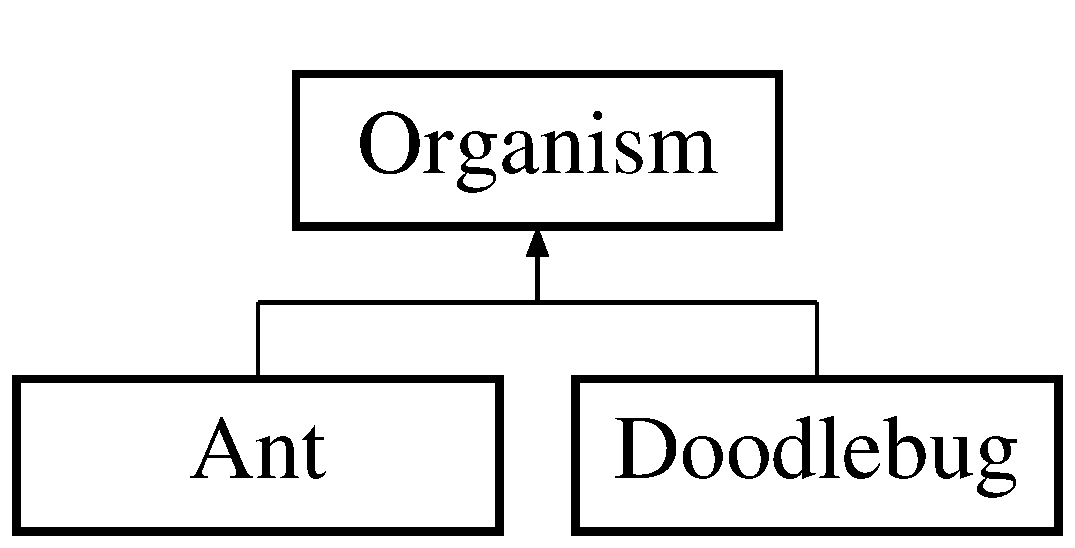
\includegraphics[height=2.000000cm]{classOrganism}
\end{center}
\end{figure}
\subsection*{Data Structures}
\begin{DoxyCompactItemize}
\item 
struct \textbf{ Coordinates}
\end{DoxyCompactItemize}
\subsection*{Public Member Functions}
\begin{DoxyCompactItemize}
\item 
\textbf{ Organism} ()
\item 
\textbf{ Organism} (bool b)
\item 
bool \textbf{ is\+Prey} ()
\item 
virtual bool \textbf{ move} ()=0
\item 
virtual bool \textbf{ breed} ()=0
\item 
virtual bool \textbf{ step} ()=0
\item 
void \textbf{ set\+Am\+Ant} (bool b)
\item 
virtual \textbf{ $\sim$\+Organism} ()
\item 
virtual int \textbf{ num\+Poss\+Cells} (int row, int col, \textbf{ Grid} $\ast$g)
\item 
virtual struct \textbf{ Coordinates} \textbf{ get\+Rand\+Cell} (int row, int col, \textbf{ Grid} $\ast$g)
\end{DoxyCompactItemize}
\subsection*{Private Attributes}
\begin{DoxyCompactItemize}
\item 
bool \textbf{ am\+Ant} = false
\end{DoxyCompactItemize}


\subsection{Constructor \& Destructor Documentation}
\mbox{\label{classOrganism_aeb16ee24b64839584b4862384d0b53fe}} 
\index{Organism@{Organism}!Organism@{Organism}}
\index{Organism@{Organism}!Organism@{Organism}}
\subsubsection{Organism()\hspace{0.1cm}{\footnotesize\ttfamily [1/2]}}
{\footnotesize\ttfamily Organism\+::\+Organism (\begin{DoxyParamCaption}{ }\end{DoxyParamCaption})}

\doxyref{Organism\+::\+Organism()}{p.}{classOrganism_aeb16ee24b64839584b4862384d0b53fe} is default constructor for a \doxyref{Organism}{p.}{classOrganism} 
\begin{DoxyParams}{Parameters}
{\em none} & \\
\hline
\end{DoxyParams}
\begin{DoxyReturn}{Returns}
none 
\end{DoxyReturn}
\mbox{\label{classOrganism_ac7d3dbebaf5df39d0a7883b2d76b4868}} 
\index{Organism@{Organism}!Organism@{Organism}}
\index{Organism@{Organism}!Organism@{Organism}}
\subsubsection{Organism()\hspace{0.1cm}{\footnotesize\ttfamily [2/2]}}
{\footnotesize\ttfamily Organism\+::\+Organism (\begin{DoxyParamCaption}\item[{bool}]{b }\end{DoxyParamCaption})}

\doxyref{Organism\+::\+Organism()}{p.}{classOrganism_aeb16ee24b64839584b4862384d0b53fe} is the Secondary Constructor 
\begin{DoxyParams}{Parameters}
{\em bool} & b is whether the organism is an ant \\
\hline
\end{DoxyParams}
\begin{DoxyReturn}{Returns}
none 
\end{DoxyReturn}


References am\+Ant.

\mbox{\label{classOrganism_aa5aa2e9fc3134358c929fa0c9d230c3b}} 
\index{Organism@{Organism}!````~Organism@{$\sim$\+Organism}}
\index{````~Organism@{$\sim$\+Organism}!Organism@{Organism}}
\subsubsection{$\sim$\+Organism()}
{\footnotesize\ttfamily Organism\+::$\sim$\+Organism (\begin{DoxyParamCaption}{ }\end{DoxyParamCaption})\hspace{0.3cm}{\ttfamily [virtual]}}

\doxyref{Organism\+::$\sim$\+Organism}{p.}{classOrganism_aa5aa2e9fc3134358c929fa0c9d230c3b} is the destructor 
\begin{DoxyParams}{Parameters}
{\em none} & \\
\hline
\end{DoxyParams}
\begin{DoxyReturn}{Returns}
none 
\end{DoxyReturn}


\subsection{Member Function Documentation}
\mbox{\label{classOrganism_a0336595710b1b4e7996852596d8be619}} 
\index{Organism@{Organism}!breed@{breed}}
\index{breed@{breed}!Organism@{Organism}}
\subsubsection{breed()}
{\footnotesize\ttfamily virtual bool Organism\+::breed (\begin{DoxyParamCaption}{ }\end{DoxyParamCaption})\hspace{0.3cm}{\ttfamily [pure virtual]}}



Implemented in \textbf{ Doodlebug} \doxyref{}{p.}{classDoodlebug_af88c6c6331094b012597ac2c688018d7}, and \textbf{ Ant} \doxyref{}{p.}{classAnt_a13f4550006f7d3626ba4c0af215e06b6}.

\mbox{\label{classOrganism_a52ff86e2ef1b525ffc5a473cfee8080e}} 
\index{Organism@{Organism}!get\+Rand\+Cell@{get\+Rand\+Cell}}
\index{get\+Rand\+Cell@{get\+Rand\+Cell}!Organism@{Organism}}
\subsubsection{get\+Rand\+Cell()}
{\footnotesize\ttfamily struct \textbf{ Organism\+::\+Coordinates} Organism\+::get\+Rand\+Cell (\begin{DoxyParamCaption}\item[{int}]{row,  }\item[{int}]{col,  }\item[{\textbf{ Grid} $\ast$}]{g }\end{DoxyParamCaption})\hspace{0.3cm}{\ttfamily [virtual]}}

Organism\+::\+Get\+Rand\+Cell() takes a grid and a row column pair, and returns a randomly picked neighboring cell with neighbors being defined as 4-\/connected 
\begin{DoxyParams}{Parameters}
{\em int} & row, the row of the cell to a get random neighboring cell from \\
\hline
{\em int} & col, the row of the cell to a get random neighboring cell from \\
\hline
{\em Grid$\ast$} & g, the grid on which you are getting the random cell \\
\hline
\end{DoxyParams}
\begin{DoxyReturn}{Returns}
output, a Coordinate struct, which contains the row, column coordinates of the random neighboring cell 
\end{DoxyReturn}


Reimplemented in \textbf{ Doodlebug} \doxyref{}{p.}{classDoodlebug_a4e8a8ced92f0624cb6ca8e1103f5c435}, and \textbf{ Ant} \doxyref{}{p.}{classAnt_a3889cd201fe6a10eabd47b90a28045ce}.



References Organism\+::\+Coordinates\+::cell\+Col, Organism\+::\+Coordinates\+::cell\+Row, empty, and num\+Poss\+Cells().



Referenced by Doodlebug\+::breed\+Doodle(), and Doodlebug\+::move().

\mbox{\label{classOrganism_aa5213b2e2b0c4f227dc7dfc4c4ab411c}} 
\index{Organism@{Organism}!is\+Prey@{is\+Prey}}
\index{is\+Prey@{is\+Prey}!Organism@{Organism}}
\subsubsection{is\+Prey()}
{\footnotesize\ttfamily bool Organism\+::is\+Prey (\begin{DoxyParamCaption}{ }\end{DoxyParamCaption})}

\doxyref{Organism\+::is\+Prey()}{p.}{classOrganism_aa5213b2e2b0c4f227dc7dfc4c4ab411c} is a function used to tell if an organism is prey 
\begin{DoxyParams}{Parameters}
{\em none} & \\
\hline
\end{DoxyParams}
\begin{DoxyReturn}{Returns}
bool returns if the organism is an ant 
\end{DoxyReturn}


References am\+Ant.

\mbox{\label{classOrganism_a9b6a5dadbe12711fa252bbfbfb988545}} 
\index{Organism@{Organism}!move@{move}}
\index{move@{move}!Organism@{Organism}}
\subsubsection{move()}
{\footnotesize\ttfamily virtual bool Organism\+::move (\begin{DoxyParamCaption}{ }\end{DoxyParamCaption})\hspace{0.3cm}{\ttfamily [pure virtual]}}



Implemented in \textbf{ Doodlebug} \doxyref{}{p.}{classDoodlebug_a4afc8c16ffb84af86ae512109bda9823}, and \textbf{ Ant} \doxyref{}{p.}{classAnt_a4aa0576c34e25ca4df23f90a3caef0f5}.

\mbox{\label{classOrganism_a00f925605ee32d2e872480e878a8848a}} 
\index{Organism@{Organism}!num\+Poss\+Cells@{num\+Poss\+Cells}}
\index{num\+Poss\+Cells@{num\+Poss\+Cells}!Organism@{Organism}}
\subsubsection{num\+Poss\+Cells()}
{\footnotesize\ttfamily int Organism\+::num\+Poss\+Cells (\begin{DoxyParamCaption}\item[{int}]{row,  }\item[{int}]{col,  }\item[{\textbf{ Grid} $\ast$}]{g }\end{DoxyParamCaption})\hspace{0.3cm}{\ttfamily [virtual]}}

\doxyref{Organism\+::num\+Poss\+Cells}{p.}{classOrganism_a00f925605ee32d2e872480e878a8848a} checks how many cells neighboring a cell are empty and returns the count of all the empty neighbors 
\begin{DoxyParams}{Parameters}
{\em int} & row, the row that this cell is on \\
\hline
{\em int} & col, the column that this cell is on \\
\hline
{\em Grid$\ast$} & g, is the grid of cells \\
\hline
\end{DoxyParams}
\begin{DoxyReturn}{Returns}
int the number of empty neighbors 
\end{DoxyReturn}


Reimplemented in \textbf{ Doodlebug} \doxyref{}{p.}{classDoodlebug_a20b30de62e78f4c27f36eaa28703b000}.



References empty, Grid\+::get\+Cell\+Occupant(), and Grid\+::get\+Num\+Cells().



Referenced by Ant\+::get\+Rand\+Cell(), get\+Rand\+Cell(), Tests2\+::organism\+Neighbor\+Test(), Tests2\+::\+Organism\+Test(), Ant\+::step(), and Doodlebug\+::step().

\mbox{\label{classOrganism_aba68f4745f6b0938cf157dcd27df1868}} 
\index{Organism@{Organism}!set\+Am\+Ant@{set\+Am\+Ant}}
\index{set\+Am\+Ant@{set\+Am\+Ant}!Organism@{Organism}}
\subsubsection{set\+Am\+Ant()}
{\footnotesize\ttfamily void Organism\+::set\+Am\+Ant (\begin{DoxyParamCaption}\item[{bool}]{b }\end{DoxyParamCaption})}

\doxyref{Organism\+::set\+Am\+Ant()}{p.}{classOrganism_aba68f4745f6b0938cf157dcd27df1868} is a function used to set if an organism is an ant 
\begin{DoxyParams}{Parameters}
{\em bool} & b, the status of the organism, true if ant false otherwise \\
\hline
\end{DoxyParams}
\begin{DoxyReturn}{Returns}
void 
\end{DoxyReturn}


References am\+Ant.

\mbox{\label{classOrganism_ae889d5671066bccdfbc15c7f16eab20e}} 
\index{Organism@{Organism}!step@{step}}
\index{step@{step}!Organism@{Organism}}
\subsubsection{step()}
{\footnotesize\ttfamily virtual bool Organism\+::step (\begin{DoxyParamCaption}{ }\end{DoxyParamCaption})\hspace{0.3cm}{\ttfamily [pure virtual]}}



Implemented in \textbf{ Doodlebug} \doxyref{}{p.}{classDoodlebug_ac6d2bbf5abc5262896a31f5b93c3a887}, and \textbf{ Ant} \doxyref{}{p.}{classAnt_ae7bb9517e9090218401d83fa2858561a}.



Referenced by Production\+::run\+Production().



\subsection{Field Documentation}
\mbox{\label{classOrganism_ab9742ed0a29e19e3c52ba74bdea66b51}} 
\index{Organism@{Organism}!am\+Ant@{am\+Ant}}
\index{am\+Ant@{am\+Ant}!Organism@{Organism}}
\subsubsection{am\+Ant}
{\footnotesize\ttfamily bool Organism\+::am\+Ant = false\hspace{0.3cm}{\ttfamily [private]}}



Referenced by is\+Prey(), Organism(), and set\+Am\+Ant().



The documentation for this class was generated from the following files\+:\begin{DoxyCompactItemize}
\item 
\textbf{ Organism.\+h}\item 
\textbf{ Organism.\+cpp}\end{DoxyCompactItemize}

\section{Production Class Reference}
\label{classProduction}\index{Production@{Production}}


{\ttfamily \#include $<$Production.\+h$>$}

\subsection*{Public Member Functions}
\begin{DoxyCompactItemize}
\item 
\textbf{ Production} (int argc, char $\ast$argv[$\,$])
\item 
bool \textbf{ run\+Production} ()
\item 
virtual \textbf{ $\sim$\+Production} ()
\item 
\textbf{ Grid} $\ast$ \textbf{ get\+Grid} ()
\end{DoxyCompactItemize}
\subsection*{Data Fields}
\begin{DoxyCompactItemize}
\item 
\textbf{ Grid} $\ast$ \textbf{ g} = nullptr
\item 
int \textbf{ time\+Steps\+Left} = 100
\end{DoxyCompactItemize}


\subsection{Constructor \& Destructor Documentation}
\mbox{\label{classProduction_a24439558b7672feaea80dc0ab1b53ff2}} 
\index{Production@{Production}!Production@{Production}}
\index{Production@{Production}!Production@{Production}}
\subsubsection{Production()}
{\footnotesize\ttfamily Production\+::\+Production (\begin{DoxyParamCaption}\item[{int}]{argc,  }\item[{char $\ast$}]{argv[$\,$] }\end{DoxyParamCaption})}

\doxyref{Production}{p.}{classProduction} Constructor 
\begin{DoxyParams}{Parameters}
{\em int} & argc is the number of parameters for the production \\
\hline
{\em char$\ast$} & argv[] is all of the arguments that we get from the console \\
\hline
\end{DoxyParams}


References ant, doodlebug, empty, g, Grid\+::print\+Grid(), Grid\+::set\+Cell\+Occupant(), Grid\+::set\+Cell\+Organism(), Grid\+::set\+Num\+Ant(), Grid\+::set\+Num\+Doodle(), Grid\+::set\+Pause(), and time\+Steps\+Left.



Referenced by main().

\mbox{\label{classProduction_ab5b3060f9e0a2bc189844e426d693dab}} 
\index{Production@{Production}!````~Production@{$\sim$\+Production}}
\index{````~Production@{$\sim$\+Production}!Production@{Production}}
\subsubsection{$\sim$\+Production()}
{\footnotesize\ttfamily Production\+::$\sim$\+Production (\begin{DoxyParamCaption}{ }\end{DoxyParamCaption})\hspace{0.3cm}{\ttfamily [virtual]}}

\doxyref{Production\+::$\sim$\+Production}{p.}{classProduction_ab5b3060f9e0a2bc189844e426d693dab} Destrcutor 
\begin{DoxyParams}{Parameters}
{\em none} & \\
\hline
\end{DoxyParams}
\begin{DoxyReturn}{Returns}
none 
\end{DoxyReturn}


Referenced by main().



\subsection{Member Function Documentation}
\mbox{\label{classProduction_a9ece57591258ca076cc9d53549dc21db}} 
\index{Production@{Production}!get\+Grid@{get\+Grid}}
\index{get\+Grid@{get\+Grid}!Production@{Production}}
\subsubsection{get\+Grid()}
{\footnotesize\ttfamily \textbf{ Grid} $\ast$ Production\+::get\+Grid (\begin{DoxyParamCaption}{ }\end{DoxyParamCaption})}

\doxyref{Production\+::get\+Grid()}{p.}{classProduction_a9ece57591258ca076cc9d53549dc21db} Gets the \doxyref{Grid}{p.}{classGrid} from the \textbackslash{} \doxyref{Production}{p.}{classProduction} Object 
\begin{DoxyParams}{Parameters}
{\em none} & \\
\hline
\end{DoxyParams}
\begin{DoxyReturn}{Returns}
the grid object 
\end{DoxyReturn}


References g.

\mbox{\label{classProduction_a1d66853eafae2580089eff44f12f07ba}} 
\index{Production@{Production}!run\+Production@{run\+Production}}
\index{run\+Production@{run\+Production}!Production@{Production}}
\subsubsection{run\+Production()}
{\footnotesize\ttfamily bool Production\+::run\+Production (\begin{DoxyParamCaption}{ }\end{DoxyParamCaption})}

\doxyref{Production\+::run\+Production()}{p.}{classProduction_a1d66853eafae2580089eff44f12f07ba} runs the simulation 
\begin{DoxyParams}{Parameters}
{\em none} & \\
\hline
\end{DoxyParams}
\begin{DoxyReturn}{Returns}
bool whether the function worked 
\end{DoxyReturn}


References ant, doodlebug, empty, g, Grid\+::get\+Cell\+Occupant(), Grid\+::get\+Cell\+Organism(), Grid\+::get\+Num\+Ant(), Grid\+::get\+Num\+Cells(), Grid\+::get\+Num\+Doodle(), Grid\+::get\+Pause(), Grid\+::print\+Grid(), Organism\+::step(), and time\+Steps\+Left.



Referenced by main().



\subsection{Field Documentation}
\mbox{\label{classProduction_ac9df298c3d4156c81eef83147ca03e83}} 
\index{Production@{Production}!g@{g}}
\index{g@{g}!Production@{Production}}
\subsubsection{g}
{\footnotesize\ttfamily \textbf{ Grid}$\ast$ Production\+::g = nullptr}



Referenced by get\+Grid(), Production(), run\+Production(), and Cell\+::set\+Occupant().

\mbox{\label{classProduction_a294328eae7f8c8a99ce441567f49bf2e}} 
\index{Production@{Production}!time\+Steps\+Left@{time\+Steps\+Left}}
\index{time\+Steps\+Left@{time\+Steps\+Left}!Production@{Production}}
\subsubsection{time\+Steps\+Left}
{\footnotesize\ttfamily int Production\+::time\+Steps\+Left = 100}



Referenced by Production(), and run\+Production().



The documentation for this class was generated from the following files\+:\begin{DoxyCompactItemize}
\item 
\textbf{ Production.\+h}\item 
\textbf{ Production.\+cpp}\end{DoxyCompactItemize}

\section{Tests2 Class Reference}
\label{classTests2}\index{Tests2@{Tests2}}


{\ttfamily \#include $<$Tests2.\+h$>$}

\subsection*{Public Member Functions}
\begin{DoxyCompactItemize}
\item 
\textbf{ Tests2} ()
\item 
bool \textbf{ do\+Tests} ()
\item 
bool \textbf{ grid\+Test} ()
\item 
bool \textbf{ make\+Ants\+Test} ()
\item 
bool \textbf{ Organism\+Test} ()
\item 
bool \textbf{ ants\+Move\+Test} ()
\item 
bool \textbf{ ants\+Breed\+Test} ()
\item 
bool \textbf{ ants\+Die\+Test} ()
\item 
bool \textbf{ make\+Doodles\+Test} ()
\item 
bool \textbf{ doodle\+Move\+Test} ()
\item 
bool \textbf{ doodle\+Breed\+Test} ()
\item 
bool \textbf{ doodle\+Eat\+Test} ()
\item 
bool \textbf{ doodle\+Dietest} ()
\item 
bool \textbf{ organism\+Neighbor\+Test} ()
\item 
bool \textbf{ organism\+Rand\+Cell\+Test} ()
\item 
virtual \textbf{ $\sim$\+Tests2} ()
\end{DoxyCompactItemize}


\subsection{Constructor \& Destructor Documentation}
\mbox{\label{classTests2_a6d7d8d248dd3d544199769baa1face60}} 
\index{Tests2@{Tests2}!Tests2@{Tests2}}
\index{Tests2@{Tests2}!Tests2@{Tests2}}
\subsubsection{Tests2()}
{\footnotesize\ttfamily Tests2\+::\+Tests2 (\begin{DoxyParamCaption}{ }\end{DoxyParamCaption})}

\mbox{\label{classTests2_abed1a850ef511b7c06ae418cb3bbd5d9}} 
\index{Tests2@{Tests2}!````~Tests2@{$\sim$\+Tests2}}
\index{````~Tests2@{$\sim$\+Tests2}!Tests2@{Tests2}}
\subsubsection{$\sim$\+Tests2()}
{\footnotesize\ttfamily Tests2\+::$\sim$\+Tests2 (\begin{DoxyParamCaption}{ }\end{DoxyParamCaption})\hspace{0.3cm}{\ttfamily [virtual]}}



Referenced by main().



\subsection{Member Function Documentation}
\mbox{\label{classTests2_a21e7692afbdfb694caf370670cbeb7d4}} 
\index{Tests2@{Tests2}!ants\+Breed\+Test@{ants\+Breed\+Test}}
\index{ants\+Breed\+Test@{ants\+Breed\+Test}!Tests2@{Tests2}}
\subsubsection{ants\+Breed\+Test()}
{\footnotesize\ttfamily bool Tests2\+::ants\+Breed\+Test (\begin{DoxyParamCaption}{ }\end{DoxyParamCaption})}



References ant, Ant\+::breed(), Grid\+::get\+Cell\+Occupant(), Grid\+::get\+Num\+Ant(), Grid\+::set\+Cell\+Occupant(), Grid\+::set\+Cell\+Organism(), Ant\+::$\sim$\+Ant(), and Grid\+::$\sim$\+Grid().



Referenced by do\+Tests().

\mbox{\label{classTests2_a045d58417814d72bcf4c97b2ebb51461}} 
\index{Tests2@{Tests2}!ants\+Die\+Test@{ants\+Die\+Test}}
\index{ants\+Die\+Test@{ants\+Die\+Test}!Tests2@{Tests2}}
\subsubsection{ants\+Die\+Test()}
{\footnotesize\ttfamily bool Tests2\+::ants\+Die\+Test (\begin{DoxyParamCaption}{ }\end{DoxyParamCaption})}



References ant, Grid\+::get\+Cell\+Organism(), Grid\+::set\+Cell\+Occupant(), Grid\+::set\+Cell\+Organism(), Ant\+::$\sim$\+Ant(), and Grid\+::$\sim$\+Grid().



Referenced by do\+Tests().

\mbox{\label{classTests2_a7694d2797eba6fadc40234d527f6afbe}} 
\index{Tests2@{Tests2}!ants\+Move\+Test@{ants\+Move\+Test}}
\index{ants\+Move\+Test@{ants\+Move\+Test}!Tests2@{Tests2}}
\subsubsection{ants\+Move\+Test()}
{\footnotesize\ttfamily bool Tests2\+::ants\+Move\+Test (\begin{DoxyParamCaption}{ }\end{DoxyParamCaption})}



References ant, doodlebug, Grid\+::get\+Cell\+Occupant(), Grid\+::get\+Cell\+Organism(), Ant\+::move(), Grid\+::print\+Grid(), Grid\+::set\+Cell\+Occupant(), Grid\+::set\+Cell\+Organism(), Ant\+::$\sim$\+Ant(), Doodlebug\+::$\sim$\+Doodlebug(), and Grid\+::$\sim$\+Grid().



Referenced by do\+Tests().

\mbox{\label{classTests2_a317dc926bf93038f188c999df7a85682}} 
\index{Tests2@{Tests2}!doodle\+Breed\+Test@{doodle\+Breed\+Test}}
\index{doodle\+Breed\+Test@{doodle\+Breed\+Test}!Tests2@{Tests2}}
\subsubsection{doodle\+Breed\+Test()}
{\footnotesize\ttfamily bool Tests2\+::doodle\+Breed\+Test (\begin{DoxyParamCaption}{ }\end{DoxyParamCaption})}



References Doodlebug\+::breed\+Doodle(), doodlebug, Grid\+::get\+Cell\+Occupant(), Grid\+::set\+Cell\+Occupant(), Grid\+::set\+Cell\+Organism(), Doodlebug\+::$\sim$\+Doodlebug(), and Grid\+::$\sim$\+Grid().



Referenced by do\+Tests().

\mbox{\label{classTests2_aaf403f9bb7338771173e2053ea4f95fc}} 
\index{Tests2@{Tests2}!doodle\+Dietest@{doodle\+Dietest}}
\index{doodle\+Dietest@{doodle\+Dietest}!Tests2@{Tests2}}
\subsubsection{doodle\+Dietest()}
{\footnotesize\ttfamily bool Tests2\+::doodle\+Dietest (\begin{DoxyParamCaption}{ }\end{DoxyParamCaption})}



References doodlebug, Grid\+::get\+Cell\+Organism(), Grid\+::set\+Cell\+Occupant(), Grid\+::set\+Cell\+Organism(), Doodlebug\+::$\sim$\+Doodlebug(), and Grid\+::$\sim$\+Grid().



Referenced by do\+Tests().

\mbox{\label{classTests2_ae35f30e7d95e581cc4ce1316409c71ac}} 
\index{Tests2@{Tests2}!doodle\+Eat\+Test@{doodle\+Eat\+Test}}
\index{doodle\+Eat\+Test@{doodle\+Eat\+Test}!Tests2@{Tests2}}
\subsubsection{doodle\+Eat\+Test()}
{\footnotesize\ttfamily bool Tests2\+::doodle\+Eat\+Test (\begin{DoxyParamCaption}{ }\end{DoxyParamCaption})}



References ant, doodlebug, Doodlebug\+::eat(), empty, Grid\+::get\+Cell\+Occupant(), Grid\+::set\+Cell\+Occupant(), Grid\+::set\+Cell\+Organism(), Doodlebug\+::$\sim$\+Doodlebug(), and Grid\+::$\sim$\+Grid().



Referenced by do\+Tests().

\mbox{\label{classTests2_a2143f2192836626e7214d37b504df381}} 
\index{Tests2@{Tests2}!doodle\+Move\+Test@{doodle\+Move\+Test}}
\index{doodle\+Move\+Test@{doodle\+Move\+Test}!Tests2@{Tests2}}
\subsubsection{doodle\+Move\+Test()}
{\footnotesize\ttfamily bool Tests2\+::doodle\+Move\+Test (\begin{DoxyParamCaption}{ }\end{DoxyParamCaption})}



References doodlebug, Grid\+::get\+Cell\+Occupant(), Grid\+::get\+Cell\+Organism(), Doodlebug\+::move(), Grid\+::print\+Grid(), Grid\+::set\+Cell\+Occupant(), Grid\+::set\+Cell\+Organism(), Doodlebug\+::$\sim$\+Doodlebug(), and Grid\+::$\sim$\+Grid().



Referenced by do\+Tests().

\mbox{\label{classTests2_a7392382310966597d685c8aa3a4a2f88}} 
\index{Tests2@{Tests2}!do\+Tests@{do\+Tests}}
\index{do\+Tests@{do\+Tests}!Tests2@{Tests2}}
\subsubsection{do\+Tests()}
{\footnotesize\ttfamily bool Tests2\+::do\+Tests (\begin{DoxyParamCaption}{ }\end{DoxyParamCaption})}



References ants\+Breed\+Test(), ants\+Die\+Test(), ants\+Move\+Test(), doodle\+Breed\+Test(), doodle\+Dietest(), doodle\+Eat\+Test(), doodle\+Move\+Test(), grid\+Test(), make\+Ants\+Test(), make\+Doodles\+Test(), organism\+Neighbor\+Test(), and organism\+Rand\+Cell\+Test().



Referenced by main().

\mbox{\label{classTests2_afe90de3a79c4105e63205cb8f019bbb2}} 
\index{Tests2@{Tests2}!grid\+Test@{grid\+Test}}
\index{grid\+Test@{grid\+Test}!Tests2@{Tests2}}
\subsubsection{grid\+Test()}
{\footnotesize\ttfamily bool Tests2\+::grid\+Test (\begin{DoxyParamCaption}{ }\end{DoxyParamCaption})}

Test the \doxyref{Grid}{p.}{classGrid} class by constructing a grid object and calling the get\+Cell\+Occupant() method on a random cell, then using the set\+Cell\+Occupant to ant, and checking if the get\+Cell\+Occupant returns ant, then destructs the grid \begin{DoxyReturn}{Returns}
true if the initialized grid does not have a occupant in a random cell and if once you use the setter method, the occupant status changes to the set enumeration (empty, ant or doodlebug) 
\end{DoxyReturn}


References ant, empty, Grid\+::get\+Cell\+Occupant(), Grid\+::set\+Cell\+Occupant(), and Grid\+::$\sim$\+Grid().



Referenced by do\+Tests().

\mbox{\label{classTests2_aa4d40396194cf770aa82dc11b449ea62}} 
\index{Tests2@{Tests2}!make\+Ants\+Test@{make\+Ants\+Test}}
\index{make\+Ants\+Test@{make\+Ants\+Test}!Tests2@{Tests2}}
\subsubsection{make\+Ants\+Test()}
{\footnotesize\ttfamily bool Tests2\+::make\+Ants\+Test (\begin{DoxyParamCaption}{ }\end{DoxyParamCaption})}

Test the \doxyref{Ant}{p.}{classAnt} class by constructing a grid object and setting a cell occupant to ant, then it creates an ant object \begin{DoxyReturn}{Returns}
true if the initialized grid does not have a occupant in a random cell and if once you use the setter method, the occupant status changes to the set enumeration (empty, ant or doodlebug) 
\end{DoxyReturn}


References ant, doodlebug, empty, Grid\+::get\+Cell\+Occupant(), Grid\+::set\+Cell\+Occupant(), and Ant\+::$\sim$\+Ant().



Referenced by do\+Tests().

\mbox{\label{classTests2_a0c6c7e5d60e7c6dc8799fa14e2b997b4}} 
\index{Tests2@{Tests2}!make\+Doodles\+Test@{make\+Doodles\+Test}}
\index{make\+Doodles\+Test@{make\+Doodles\+Test}!Tests2@{Tests2}}
\subsubsection{make\+Doodles\+Test()}
{\footnotesize\ttfamily bool Tests2\+::make\+Doodles\+Test (\begin{DoxyParamCaption}{ }\end{DoxyParamCaption})}



References doodlebug, empty, Grid\+::get\+Cell\+Occupant(), Grid\+::set\+Cell\+Occupant(), Doodlebug\+::$\sim$\+Doodlebug(), and Grid\+::$\sim$\+Grid().



Referenced by do\+Tests().

\mbox{\label{classTests2_a90596465639d148c48a629a00df6fec5}} 
\index{Tests2@{Tests2}!organism\+Neighbor\+Test@{organism\+Neighbor\+Test}}
\index{organism\+Neighbor\+Test@{organism\+Neighbor\+Test}!Tests2@{Tests2}}
\subsubsection{organism\+Neighbor\+Test()}
{\footnotesize\ttfamily bool Tests2\+::organism\+Neighbor\+Test (\begin{DoxyParamCaption}{ }\end{DoxyParamCaption})}



References ant, Organism\+::num\+Poss\+Cells(), Grid\+::set\+Cell\+Occupant(), and Grid\+::set\+Cell\+Organism().



Referenced by do\+Tests().

\mbox{\label{classTests2_a21837e3bc1c24819ce67bff0ed5523b9}} 
\index{Tests2@{Tests2}!organism\+Rand\+Cell\+Test@{organism\+Rand\+Cell\+Test}}
\index{organism\+Rand\+Cell\+Test@{organism\+Rand\+Cell\+Test}!Tests2@{Tests2}}
\subsubsection{organism\+Rand\+Cell\+Test()}
{\footnotesize\ttfamily bool Tests2\+::organism\+Rand\+Cell\+Test (\begin{DoxyParamCaption}{ }\end{DoxyParamCaption})}



References ant, Ant\+::\+Ant(), Organism\+::\+Coordinates\+::cell\+Col, Organism\+::\+Coordinates\+::cell\+Row, Ant\+::get\+Rand\+Cell(), Grid\+::set\+Cell\+Occupant(), and Grid\+::set\+Cell\+Organism().



Referenced by do\+Tests().

\mbox{\label{classTests2_a60ee731c9808abf3722e0e15e6037ac2}} 
\index{Tests2@{Tests2}!Organism\+Test@{Organism\+Test}}
\index{Organism\+Test@{Organism\+Test}!Tests2@{Tests2}}
\subsubsection{Organism\+Test()}
{\footnotesize\ttfamily bool Tests2\+::\+Organism\+Test (\begin{DoxyParamCaption}{ }\end{DoxyParamCaption})}



References ant, empty, Grid\+::get\+Cell\+Occupant(), Grid\+::get\+Num\+Cells(), Organism\+::num\+Poss\+Cells(), Grid\+::set\+Cell\+Occupant(), Ant\+::$\sim$\+Ant(), and Grid\+::$\sim$\+Grid().



The documentation for this class was generated from the following files\+:\begin{DoxyCompactItemize}
\item 
\textbf{ Tests2.\+h}\item 
\textbf{ Tests2.\+cpp}\end{DoxyCompactItemize}

\chapter{File Documentation}
\section{Ant.\+cpp File Reference}
\label{Ant_8cpp}\index{Ant.\+cpp@{Ant.\+cpp}}
{\ttfamily \#include \char`\"{}Ant.\+h\char`\"{}}\newline
{\ttfamily \#include \char`\"{}Grid.\+h\char`\"{}}\newline
{\ttfamily \#include $<$stdlib.\+h$>$}\newline
{\ttfamily \#include $<$stdio.\+h$>$}\newline

\section{Ant.\+h File Reference}
\label{Ant_8h}\index{Ant.\+h@{Ant.\+h}}
{\ttfamily \#include \char`\"{}Organism.\+h\char`\"{}}\newline
{\ttfamily \#include \char`\"{}Grid.\+h\char`\"{}}\newline
\subsection*{Data Structures}
\begin{DoxyCompactItemize}
\item 
class \textbf{ Ant}
\end{DoxyCompactItemize}

\section{Ants\+And\+Doodles.\+cpp File Reference}
\label{AntsAndDoodles_8cpp}\index{Ants\+And\+Doodles.\+cpp@{Ants\+And\+Doodles.\+cpp}}
{\ttfamily \#include $<$iostream$>$}\newline
{\ttfamily \#include \char`\"{}Tests2.\+h\char`\"{}}\newline
{\ttfamily \#include \char`\"{}Production.\+h\char`\"{}}\newline
\subsection*{Functions}
\begin{DoxyCompactItemize}
\item 
int \textbf{ main} (int argc, char $\ast$argv[$\,$])
\end{DoxyCompactItemize}


\subsection{Function Documentation}
\mbox{\label{AntsAndDoodles_8cpp_a0ddf1224851353fc92bfbff6f499fa97}} 
\index{Ants\+And\+Doodles.\+cpp@{Ants\+And\+Doodles.\+cpp}!main@{main}}
\index{main@{main}!Ants\+And\+Doodles.\+cpp@{Ants\+And\+Doodles.\+cpp}}
\subsubsection{main()}
{\footnotesize\ttfamily int main (\begin{DoxyParamCaption}\item[{int}]{argc,  }\item[{char $\ast$}]{argv[$\,$] }\end{DoxyParamCaption})}



References Tests2\+::do\+Tests(), Production\+::\+Production(), Production\+::run\+Production(), Production\+::$\sim$\+Production(), and Tests2\+::$\sim$\+Tests2().


\section{Cell.\+cpp File Reference}
\label{Cell_8cpp}\index{Cell.\+cpp@{Cell.\+cpp}}
{\ttfamily \#include \char`\"{}Cell.\+h\char`\"{}}\newline
{\ttfamily \#include \char`\"{}Organism.\+h\char`\"{}}\newline

\section{Cell.\+h File Reference}
\label{Cell_8h}\index{Cell.\+h@{Cell.\+h}}
\subsection*{Data Structures}
\begin{DoxyCompactItemize}
\item 
class \textbf{ Cell}
\end{DoxyCompactItemize}
\subsection*{Enumerations}
\begin{DoxyCompactItemize}
\item 
enum \textbf{ occupation\+Status} \{ \textbf{ empty}, 
\textbf{ ant}, 
\textbf{ doodlebug}
 \}
\end{DoxyCompactItemize}


\subsection{Enumeration Type Documentation}
\mbox{\label{Cell_8h_abcce8bf608a2504bf718b7234aa15acb}} 
\index{Cell.\+h@{Cell.\+h}!occupation\+Status@{occupation\+Status}}
\index{occupation\+Status@{occupation\+Status}!Cell.\+h@{Cell.\+h}}
\subsubsection{occupation\+Status}
{\footnotesize\ttfamily enum \textbf{ occupation\+Status}}

\begin{DoxyEnumFields}{Enumerator}
\raisebox{\heightof{T}}[0pt][0pt]{\index{empty@{empty}!Cell.\+h@{Cell.\+h}}\index{Cell.\+h@{Cell.\+h}!empty@{empty}}}\mbox{\label{Cell_8h_abcce8bf608a2504bf718b7234aa15acbae8654263bd8adf1d0922f427d8f3fc1b}} 
empty&\\
\hline

\raisebox{\heightof{T}}[0pt][0pt]{\index{ant@{ant}!Cell.\+h@{Cell.\+h}}\index{Cell.\+h@{Cell.\+h}!ant@{ant}}}\mbox{\label{Cell_8h_abcce8bf608a2504bf718b7234aa15acbacc8f2f9c5b15a05a2f336152b3794aa9}} 
ant&\\
\hline

\raisebox{\heightof{T}}[0pt][0pt]{\index{doodlebug@{doodlebug}!Cell.\+h@{Cell.\+h}}\index{Cell.\+h@{Cell.\+h}!doodlebug@{doodlebug}}}\mbox{\label{Cell_8h_abcce8bf608a2504bf718b7234aa15acba55f311222a925986c2589e11b469c0f2}} 
doodlebug&\\
\hline

\end{DoxyEnumFields}

\section{Doodlebug.\+cpp File Reference}
\label{Doodlebug_8cpp}\index{Doodlebug.\+cpp@{Doodlebug.\+cpp}}
{\ttfamily \#include \char`\"{}Doodlebug.\+h\char`\"{}}\newline
{\ttfamily \#include \char`\"{}Grid.\+h\char`\"{}}\newline
{\ttfamily \#include $<$stdlib.\+h$>$}\newline
{\ttfamily \#include $<$stdio.\+h$>$}\newline

\section{Doodlebug.\+h File Reference}
\label{Doodlebug_8h}\index{Doodlebug.\+h@{Doodlebug.\+h}}
{\ttfamily \#include \char`\"{}Organism.\+h\char`\"{}}\newline
{\ttfamily \#include \char`\"{}Grid.\+h\char`\"{}}\newline
{\ttfamily \#include \char`\"{}Ant.\+h\char`\"{}}\newline
\subsection*{Data Structures}
\begin{DoxyCompactItemize}
\item 
class \textbf{ Doodlebug}
\end{DoxyCompactItemize}

\section{Grid.\+cpp File Reference}
\label{Grid_8cpp}\index{Grid.\+cpp@{Grid.\+cpp}}
{\ttfamily \#include $<$iostream$>$}\newline
{\ttfamily \#include $<$iomanip$>$}\newline
{\ttfamily \#include \char`\"{}Grid.\+h\char`\"{}}\newline
{\ttfamily \#include \char`\"{}Cell.\+h\char`\"{}}\newline

\section{Grid.\+h File Reference}
\label{Grid_8h}\index{Grid.\+h@{Grid.\+h}}
{\ttfamily \#include \char`\"{}Cell.\+h\char`\"{}}\newline
\subsection*{Data Structures}
\begin{DoxyCompactItemize}
\item 
class \textbf{ Grid}
\end{DoxyCompactItemize}

\section{Organism.\+cpp File Reference}
\label{Organism_8cpp}\index{Organism.\+cpp@{Organism.\+cpp}}
{\ttfamily \#include \char`\"{}Organism.\+h\char`\"{}}\newline
{\ttfamily \#include \char`\"{}Grid.\+h\char`\"{}}\newline
{\ttfamily \#include \char`\"{}Cell.\+h\char`\"{}}\newline
{\ttfamily \#include $<$stdlib.\+h$>$}\newline

\section{Organism.\+h File Reference}
\label{Organism_8h}\index{Organism.\+h@{Organism.\+h}}
{\ttfamily \#include \char`\"{}Grid.\+h\char`\"{}}\newline
{\ttfamily \#include $<$stdlib.\+h$>$}\newline
{\ttfamily \#include $<$stdio.\+h$>$}\newline
\subsection*{Data Structures}
\begin{DoxyCompactItemize}
\item 
class \textbf{ Organism}
\item 
struct \textbf{ Organism\+::\+Coordinates}
\end{DoxyCompactItemize}

\section{Production.\+cpp File Reference}
\label{Production_8cpp}\index{Production.\+cpp@{Production.\+cpp}}
{\ttfamily \#include $<$iostream$>$}\newline
{\ttfamily \#include $<$algorithm$>$}\newline
{\ttfamily \#include $<$stdio.\+h$>$}\newline
{\ttfamily \#include $<$stdlib.\+h$>$}\newline
{\ttfamily \#include $<$time.\+h$>$}\newline
{\ttfamily \#include \char`\"{}Production.\+h\char`\"{}}\newline
{\ttfamily \#include \char`\"{}Grid.\+h\char`\"{}}\newline
{\ttfamily \#include \char`\"{}Cell.\+h\char`\"{}}\newline
{\ttfamily \#include \char`\"{}Organism.\+h\char`\"{}}\newline
{\ttfamily \#include \char`\"{}Doodlebug.\+h\char`\"{}}\newline
{\ttfamily \#include \char`\"{}Ant.\+h\char`\"{}}\newline

\section{Production.\+h File Reference}
\label{Production_8h}\index{Production.\+h@{Production.\+h}}
{\ttfamily \#include \char`\"{}Grid.\+h\char`\"{}}\newline
\subsection*{Data Structures}
\begin{DoxyCompactItemize}
\item 
class \textbf{ Production}
\end{DoxyCompactItemize}

\section{Tests2.\+cpp File Reference}
\label{Tests2_8cpp}\index{Tests2.\+cpp@{Tests2.\+cpp}}
{\ttfamily \#include \char`\"{}Tests2.\+h\char`\"{}}\newline
{\ttfamily \#include \char`\"{}Grid.\+h\char`\"{}}\newline
{\ttfamily \#include \char`\"{}Ant.\+h\char`\"{}}\newline
{\ttfamily \#include \char`\"{}Doodlebug.\+h\char`\"{}}\newline
{\ttfamily \#include \char`\"{}Cell.\+h\char`\"{}}\newline
{\ttfamily \#include $<$iostream$>$}\newline
{\ttfamily \#include $<$stdio.\+h$>$}\newline

\section{Tests2.\+h File Reference}
\label{Tests2_8h}\index{Tests2.\+h@{Tests2.\+h}}
\subsection*{Data Structures}
\begin{DoxyCompactItemize}
\item 
class \textbf{ Tests2}
\end{DoxyCompactItemize}

%--- End generated contents ---

% Index
\backmatter
\newpage
\phantomsection
\clearemptydoublepage
\addcontentsline{toc}{chapter}{Index}
\printindex

\end{document}
